\documentclass[12pt]{article}
\usepackage[utf8]{inputenc}
\usepackage{enumitem}
\usepackage{graphicx}
\usepackage[margin=1in]{geometry}
\usepackage{amsmath}
\usepackage{amssymb}
\usepackage{mathtools}
\usepackage{authblk}
\usepackage{hyperref}
\usepackage[ruled,vlined]{algorithm2e}
\usepackage{subcaption}

\hypersetup{
    colorlinks=true,
    linkcolor=blue,
    filecolor=magenta,      
    urlcolor=cyan,
}

%\setlength{\parskip}{1em}
\title{Capturing patterns of variation unique to a specific dataset}
\author[1]{Robin Tu}
\author[2]{Alexander H. Foss}
\author[1]{Sihai Dave Zhao}
\affil[1]{Department of Statistics, University of Illinois at Urbana-Champaign, Champaign, IL}
\affil[2]{Statistical Sciences, Sandia National Laboratories, Albuquerque, NM}

%\date{August 2020}

\begin{document}

\maketitle

\section{Introduction}

Capturing patterns of variation present in a dataset is an important step in exploratory data analysis and unsupervised learning. Popular methods include principal component analysis (PCA) \cite{pca}, nonnegative matrix factorization \cite{Lee1999}, projection pursuit \cite{pp}, and independent component analysis \cite{ica}. Frequently, however, many of the identified patterns may actually arise from systematic or technical variation, for example batch effects, that are not of substantive interest.

New approaches are necessary for capturing meaningful patterns of variation. A popular approach is to contrast a target dataset of interest with a carefully chosen background dataset that represents unwanted or uninteresting variation. Patterns of variation unique to the target, and not present in the background, are more likely to be substantively meaningful.
For example, in Section \ref{sec:mouse}, we analyze proteomics data from of normal and trisomic mice that have undergone Context Shock treatment and/or drug therapy. One goal is to identify patterns uniquely associated with normal mice. However, the dominant modes of variation in the dataset arise from the Context Shock treatment and the trisomic gene, which are not of interest. Therefore, we contrast the data with a background dataset of proteomics data from Context Shock-treated and drug-treated trisomic mice. As a result, the remaining patterns of variation unique to the target dataset reveal features specific to normal mice.
%For example, in Section \ref{sec:faces}, we analyze images of the faces of actors expressing different emotions. Our goal is to identify features uniquely associated with expression of fear (labeled as afraid). However, the dominant modes of variation in the dataset correspond to general variation in facial features that are not meaningful for the emotion of interest. Therefore, we contrast the data with a background dataset of images of other emotions that are not of interest. As a result, the remaining patterns of variation unique to the target dataset reveal features specific to afraid.

This approach was first introduced by Abid et al. \cite{Abid}, who proposed contrastive principal components analysis (cPCA). While standard PCA identifies directions of variation that explain the most variation in the target dataset, cPCA seeks directions that explain more variation in the target than in the background. The most important patterns are those corresponding to the largest gap between the two datasets. Salloum and Kuo \cite{Salloum} later introduced cPCA++, which maximizes the ratio, rather than the difference, of the variance explained by the target and background. Boileau et al. \cite{Boileau} described sparse cPCA, which seeks maxmially contrastive patterns of variation that can be characterized using a parsimonious set of features. Other types of contrastive implementations include latent models \cite{severson2019unsupervised} and autoencoders \cite{cautoencoder}.

There are two main issues with existing contrastive methods. First, a major disadvantage is that they cannot accommodate multiple background datasets. Using multiple backgrounds allows researchers to better hone in on the unique variation of interest by removing multiple types or sources of unwanted variation.
%referencing section faces is awkward cause we never talk about mice. should we do mice too?
For example, in the emotion analysis in Section \ref{sec:faces}, where we seek to uncover facial features characterizing the expression of ``afraid'', the dataset we use also contains background images from six other emotions. If we can simultaneously contrast the target data with multiple other background emotions, we will be able to identify more refined and distinctive patterns of variation characterizing ``afraid''. Naively applying existing methods by pooling the different emotions into a single background dataset is suboptimal, as variation in the pooled data may not be representative of variation in any of the individual datasets.

The second disadvantage of existing contrastive methods is that they typically require one or more tuning parameters. For example, cPCA requires the user to specify how much to penalize patterns that explain a large amount of variation in the background data. It is not clear in general how to choose these tuning parameters objectively.

We propose Unique Component Analysis (UCA), which addresses both of these issues. % UCA works by constraining the objective function in cPCA to give directions that are orthonormal and explain small amounts of variation in each background dataset. Specifically, let $A$ be the $p \times p$ target covariance matrix and $B_j$, $j \in 1,\ldots, m$ be the $m$ $p\times p$ background covariance matrices. We seek to: 
% \begin{align}
%   &\max_{v\in \mathbb{R}^p}{v^TAv} \nonumber\\ 
%   \text{subject to }&\; v^{T}v=I,\;\; v^TB_1 v \leq 1, \ldots, v^T B_m v \leq 1 \nonumber
% \end{align}
% These constraints are naturally found in generalized eigenvalue problems and can be solved using weak duality of the Lagrangian.
Not only can UCA contrast a target dataset against multiple backgrounds, but it also does not require any tuning parameters. UCA finds directions of variation that maximize the explained variation in the target under a constraint on the amount of variation they can explain in each of the backgrounds. With a single background, UCA is equivalent to cPCA but with an automatically selected tuning parameter. We show that UCA achieves similar results as cPCA and cPCA++ with a single background and that it can outperform them when using multiple backgrounds. We also develop computationally scalable algorithms for application to experiments with large numbers of measured features.
% concluding statement. feels unfinished when we just leave it at "we also developed this algo. Possibly put a big picture statment here llike a future casting of sort that we elaborate further in the conclusion


% Another way to conduct contrastive dimension reduction is with ``Residual PCA''. We note that residual PCA (rPCA) is not a formal technique but is used as an ad-hoc method of removing noise from known variability  \cite{rpca}. Again, let $A$ be the $p \times p$ target covariance matrix and $B$ be the $p\times p$ background covariance matrix.  For some integer $k$ which denotes the low dimensional representation of $B$, rPCA performs PCA after projecting $A$ onto the ``residual'' space of $B$. More specifically, if $W$ denotes the eigenvectors of $B$ and $W_{(k+1):p}$ the top $(k+1):p$ eigenvectors of $B$,then rPCA seeks to:
% \[\max_{v\in \mathbb{R}^p}{v^T \left(W_{(k+1):p}W_{(k+1):p}^T A\right) v}\]
% Note that cPCA with contrastive parameter $\lambda \rightarrow \infty$ is different from rPCA because rPCA requires user to choose the number of background components to be kept, whereas cPCA with $\lambda \rightarrow \infty$ maps reduces the target on the nullspace of the background-- they would be equivalent for $k = p$. We present rPCA to demonstrate that some of the same underlying directions can be found in a more intuitive way. It also can easily be extensible to multiple backgrounds by projecting onto addition background residual spaces. Since the residual space of the background can be done easily with singular-value decomposition, it is computationally simple and straight forward. However, one still needs to choose the background data dimension, $k$.
% To solve this tuning parameter problem, we use the elbow method of finding the best linear single knot spline at $k$ such that the mean-square error is minimized in the scree plot. For the examples below, we will default to this method of selecting $k$. %(Cite...I don't remember the citation for this...)


\section{Results}
\subsection{\label{sec:mouse}Discovering subgroups in protein expression data}
\begin{figure}[th!]
  \centering
  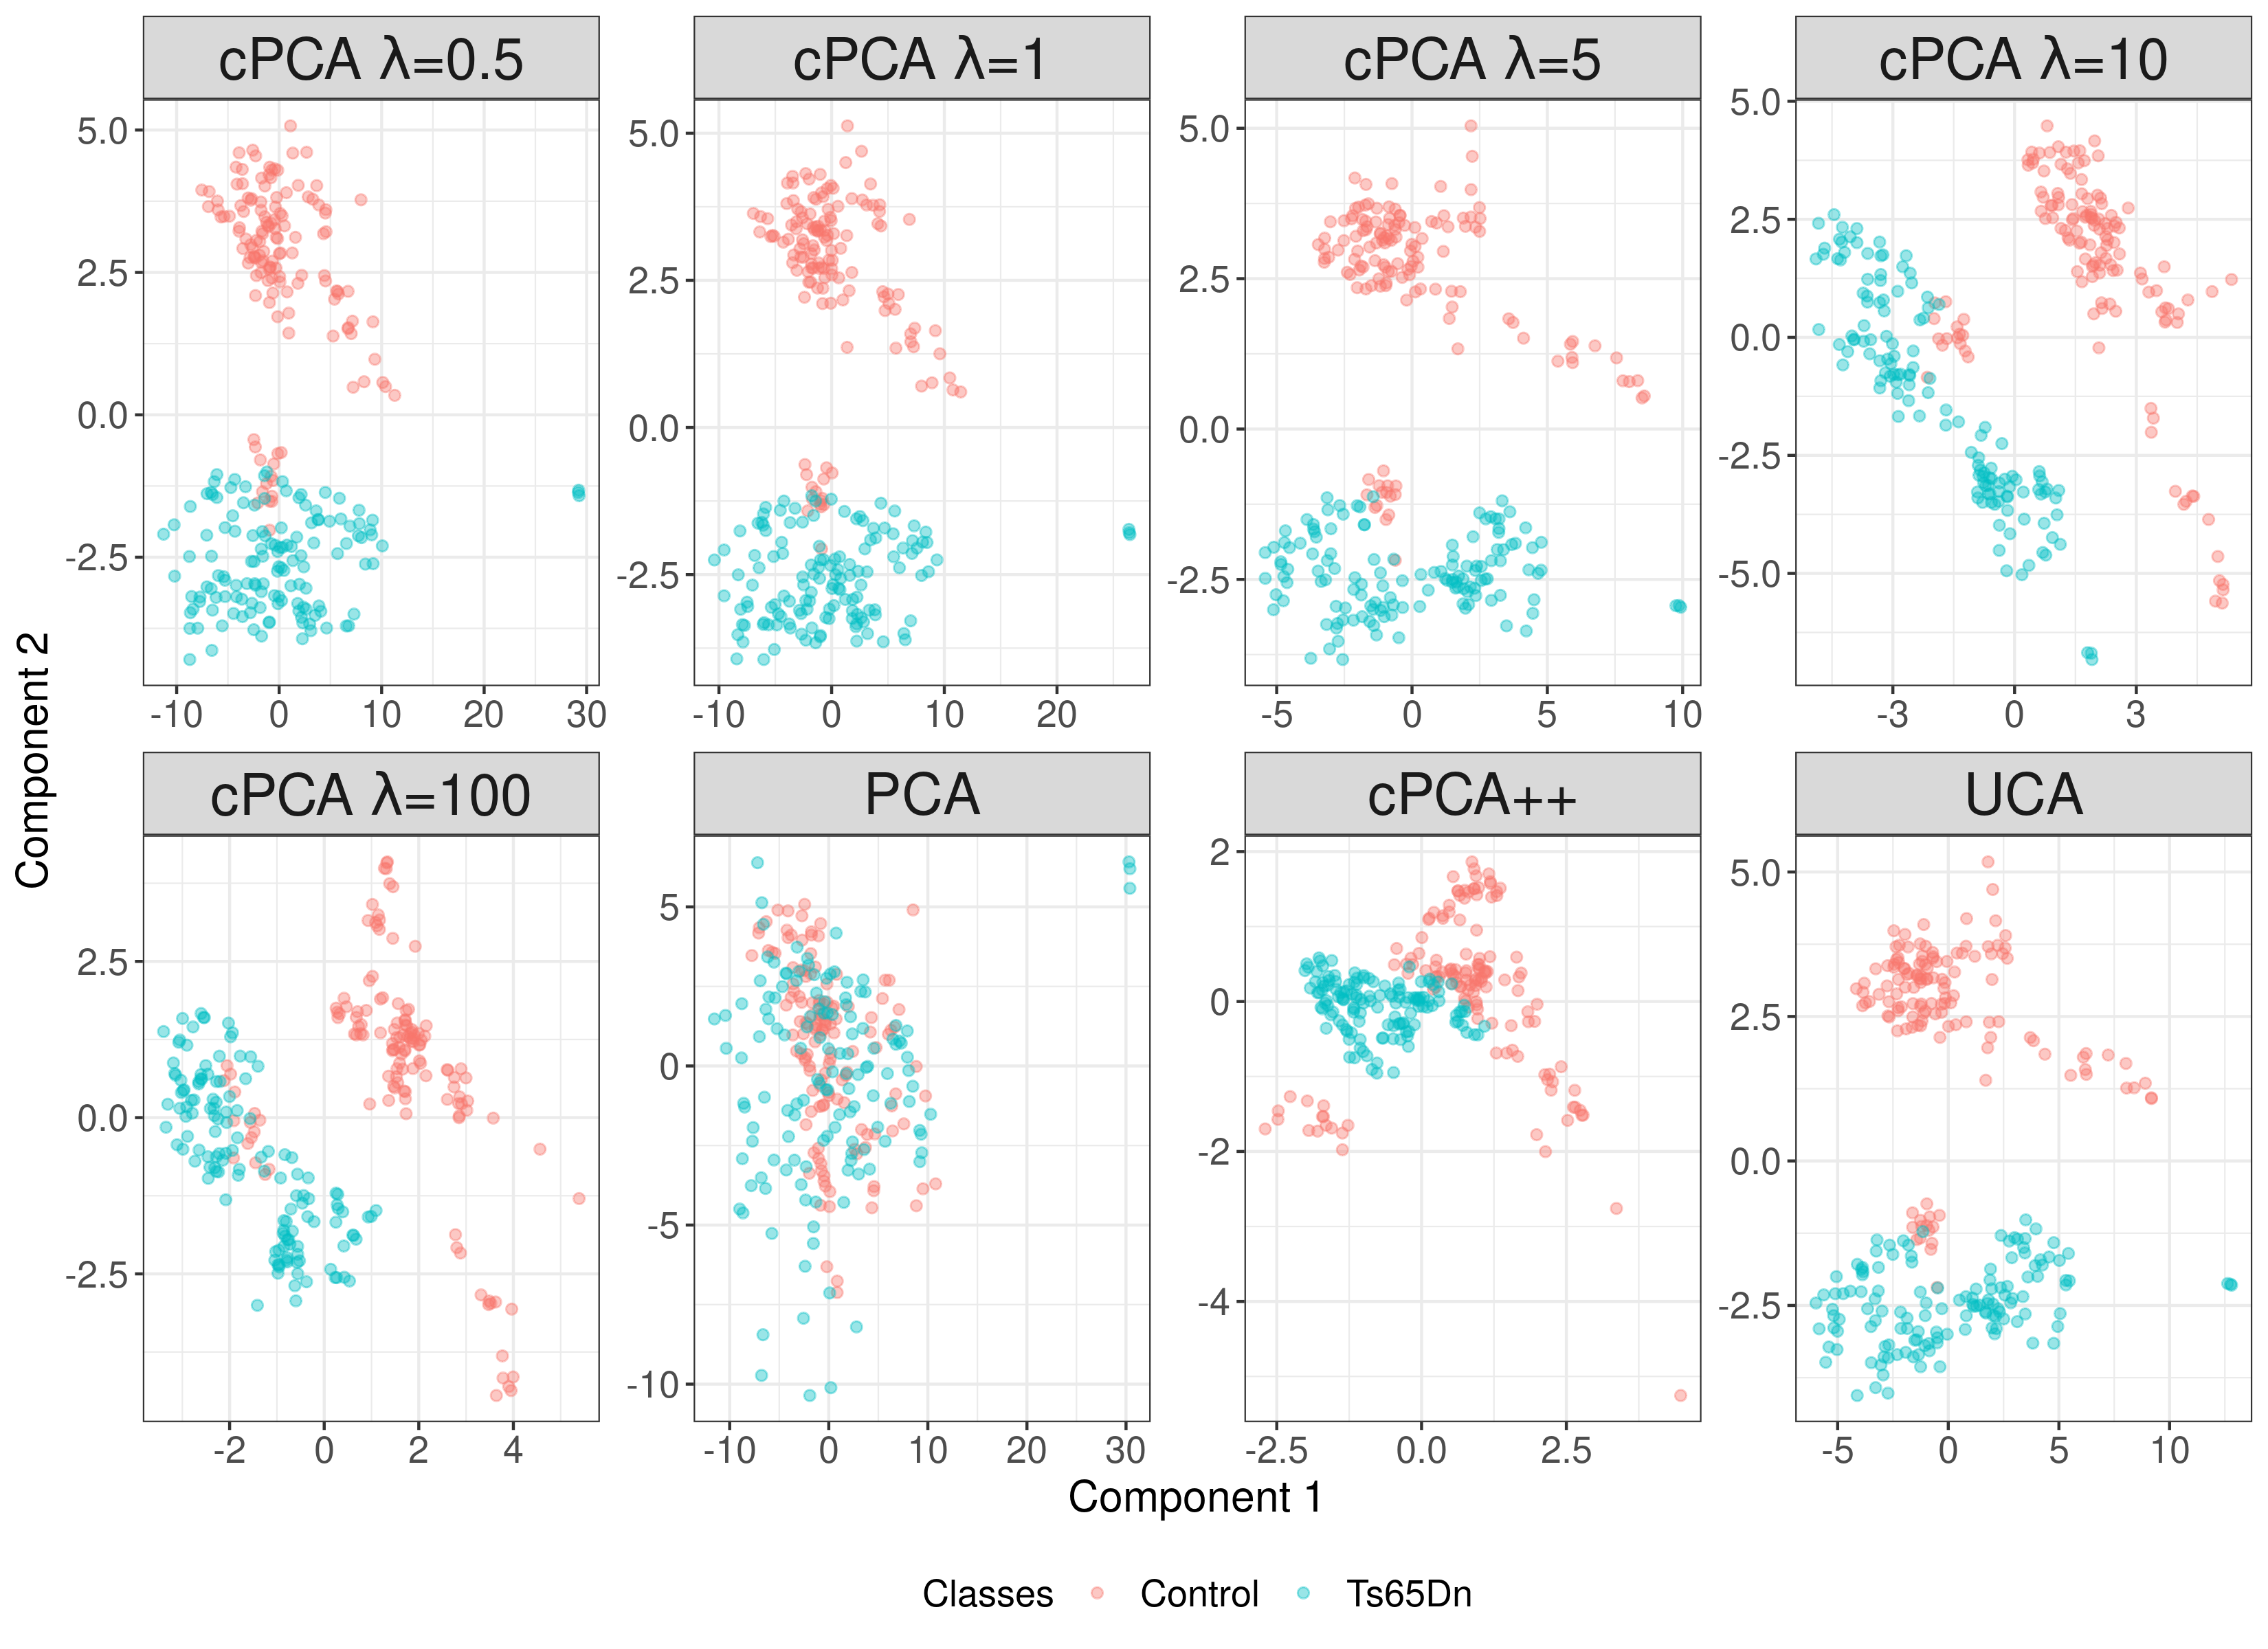
\includegraphics[width = 0.8\textwidth]{figure/Mouse_Data.png}
  \caption{Mouse Protein Expression: Down Syndrome (Ts65Dn) separability of saline injected mice which were shocked before getting environmental context (Shock Context). Both normal and trisomic mice receiving Shock Context treatment do not associate novel environments with adverse stimulus. Down Syndrome and control mice were unseparable using PCA alone but is easily separable by cPCA at all values of the contrastive parameter $\lambda$. The mice are also easily separable by cPCA++ and UCA.}
  \label{fig:Mouse}
\end{figure}

% \textbf{ I THINK YOUR ORIGINAL WRITEUP WAS BACKWARDS AND FLIPPED SHOCKED VS UNSHOCKED. ALSO, IS THE TOTAL SAMPLE SIZE OF 1080 CORRECT?}
% nope not flipped. and yes, total samples they say on the UCI database was 1080, and each sample could be treated as if they were independent even tho some measurements were repeated on the same mice. 

We applied UCA to mouse proteomics data, which were also used by Abid et al. \cite{Abid} to illustrate cPCA performance. The study measured levels of 76 proteins in 1080 normal and trisomic (Down Syndrome) mice receiving various combinations of learning therapies (Context Shock vs. Shock Context) and drug (memantine vs. saline) \cite{Ahmed, Higuera, Abid}. Normal mice exposed to Context Shock will first be exposed to novel context then shocked, and learn to associate novel contexts with adverse stimulus; trisomic mice will not learn this association. Under the Shock Context treatment, mice are first shocked than exposed to novel context, resulting in normal and trisomic mice not associating the environment with adverse stimulus. The goal of the experiment was to assess whether memantine improved learning ability in trisomic mice and to identify subsets of protein that may be involved in this process.

We first replicate the analysis by Abid et al. \cite{Abid}. We want to extract patterns of variation in protein levels that can help discriminate normal from trisomic mice. Our target dataset consisted of protein data from Shock Context mice given saline. However, natural variation, arising from factors such as age and gender, may dominant this dataset and obscure the variation of interest due to trisomy. To remove this natural variation, we contrasted the target data with a background dataset consisting of normal Context Shocked mice who had been given saline. As natural variation is likely present in both the target and the background, patterns that explaining variation in the target but not the background may be more likely to related to trisomy.

Figure \ref{fig:Mouse} shows the data projected to the first two components identified by PCA, cPCA, cPCA++, and UCA. Normal and trisomic mice are not well-separated in the PCA results, showing that dominant variation in the target data indeed does not stem from trisomy. In contrast, the two mouse groups are much more clearly separated in the cPCA results. While this separation is noticeable for each of the tuning parameter values we tried, the actual projected data can vary considerably, and the optimal tuning parameter value remains unclear.
cPCA++, which does not require specifying tuning parameter here because the number of samples exceeds the number of features, shows better separation than PCA but does not perform as well as cPCA. UCA performs as well as cPCA but without requiring a tuning parameter.

\begin{figure}[th!]
  \centering
  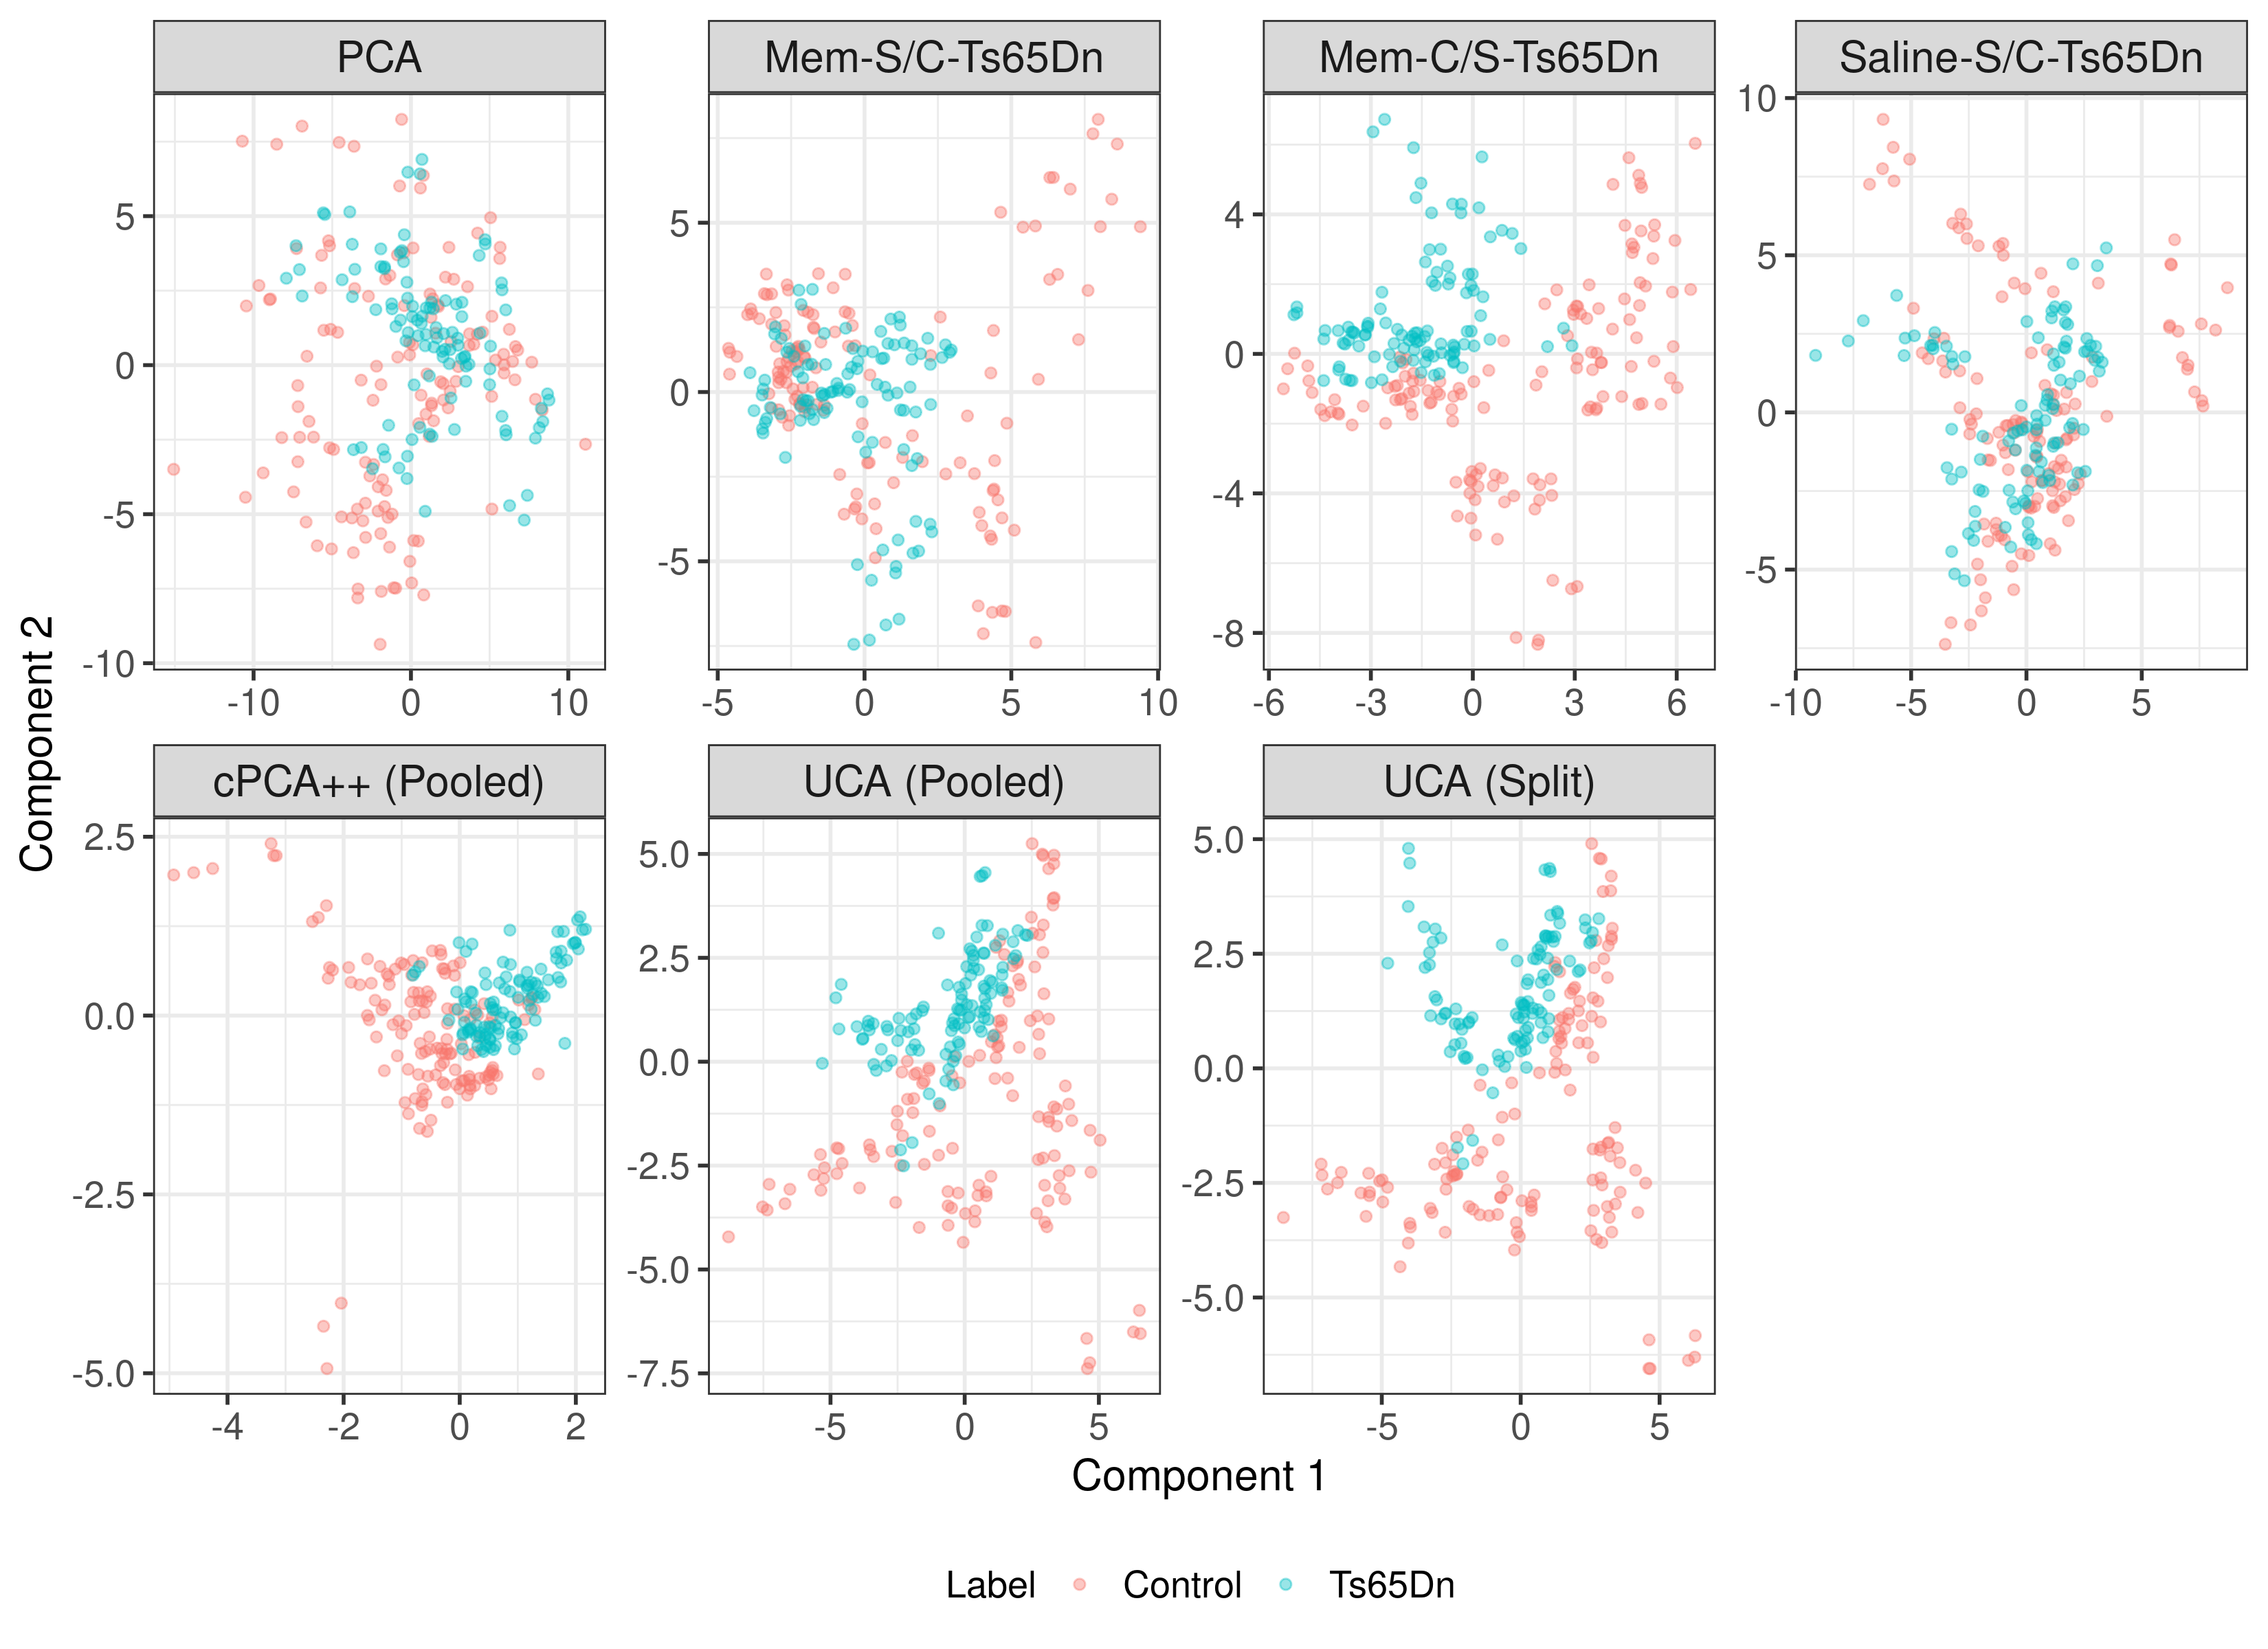
\includegraphics[width = 0.9\textwidth]{figure/Mouse_split_stack_Ts65Dn.png}
  \caption{Mouse Protein Expression: Separability of normal and trisomic Context Shocked mice injected with saline. Background datasets: Shock Contex trisomic mice injected with memantine (Mem-S/C-Ts65Dn), Context Shock trisomic mice injected with memantine (Mem-C/S-Ts65Dn), and Shock Context trisomic mice injected with saline (Saline-S/C-Ts65Dn). Pooled: all background datasets are pooled into one background. Split: UCA using multiple separate individual backgrounds.}
  \label{fig:MouseSplitStack}
\end{figure}

We next repeat the same analysis, but this time using Context Shocked mice given saline as our target dataset. Abid et al. \cite{Abid} did not consider this analysis, where separating normal and trisomic Context Shocked mice proves to be a much more challenging problem. Figure \ref{fig:MouseSplitStack} shows that normal and trisomic mice are again not well-separated by the first two components learned by PCA.
Here we extract patterns of variation unique to normal mice and so applied UCA using three trisomic mouse datasets as backgrounds.

The results show that a single background dataset alone cannot separate normal and trisomic mice well. Pooling the three individual backgrounds together achieves slightly better separability compared to some of the individual backgrounds. However, natively constrasting multiple backgrounds simultaneously without pooling allows our proposed UCA to remove variability specific to each background and results in the best separability.


%Here, we use UCA as a best case proxy for cPCA.  We note that under the shock therapy condition, cPCA with other values of the contrastive parameter result in worse separability than figure \ref{fig:MouseSplitStack} (see figure \ref{fig:mouse_stack_cpca} in the Appendix). 


% We also note that the choice of background is crucial and that not some backgrounds are unsuitable... using control instead leads to bad results?

% We show that our results match the cPCA results
% We show that cPCA depends on tuning parameter
% results of cPCA++ aren't impressive
% residual PCA yields similar results.

\subsection{\label{sec:faces}Discovering eigenfaces of emotion}

We further illustrate the advantages of contrasting multiple background datasets with UCA using the Karolinska Directed Emotional Faces (KDEF) \cite{Calvo2008}, which captured images of seven emotions from five different angles from 70 amateur actors in either a practice or final session. Figure \ref{fig:faces-mean} presents averaged images of each emotion calculated from all female actors in their final session. 

We focus on uncovering variation unique to the ``afraid'' emotion using all final session pictures from every emotion from female actors. Since this target contains six other emotions, standard PCA will not provide variation unique to ``afraid''. Instead, we leverage images from the practice session to serve as background data. We construct six separate backgrounds, corresponding to the six other emotions, and contrast out their variation using UCA. For comparison, we also pooled these images together into a single background dataset and performed UCA using the pooled background.

% \begin{figure}[th]
% \centering
% \tabskip=0pt
% \valign{#\cr
%   \hbox{%
%     \begin{subfigure}[b]{.51\textwidth}
%     \centering
%     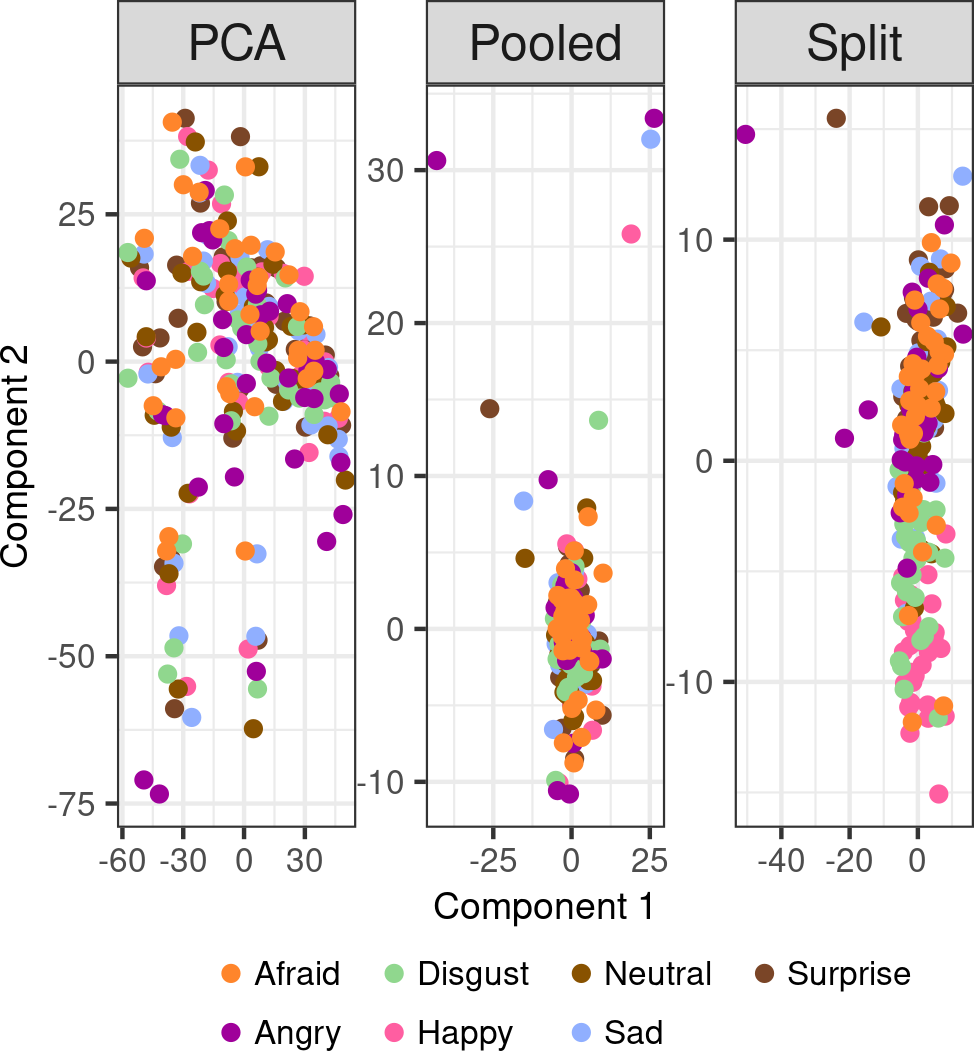
\includegraphics[height = 13.5cm,width=\textwidth]{figure/Afraid_projected_1_2_removed.png}
%     \caption{}
%     \label{fig:faces-projected}
% %Faces projected onto the first two components found by PCA, UCA with a pooled background, and UCA with backgrounds split
%     \end{subfigure}%
%   }\cr
%   \noalign{\hfill}
%   \hbox{%
%     \begin{subfigure}{.48\textwidth}
%     \centering
%     %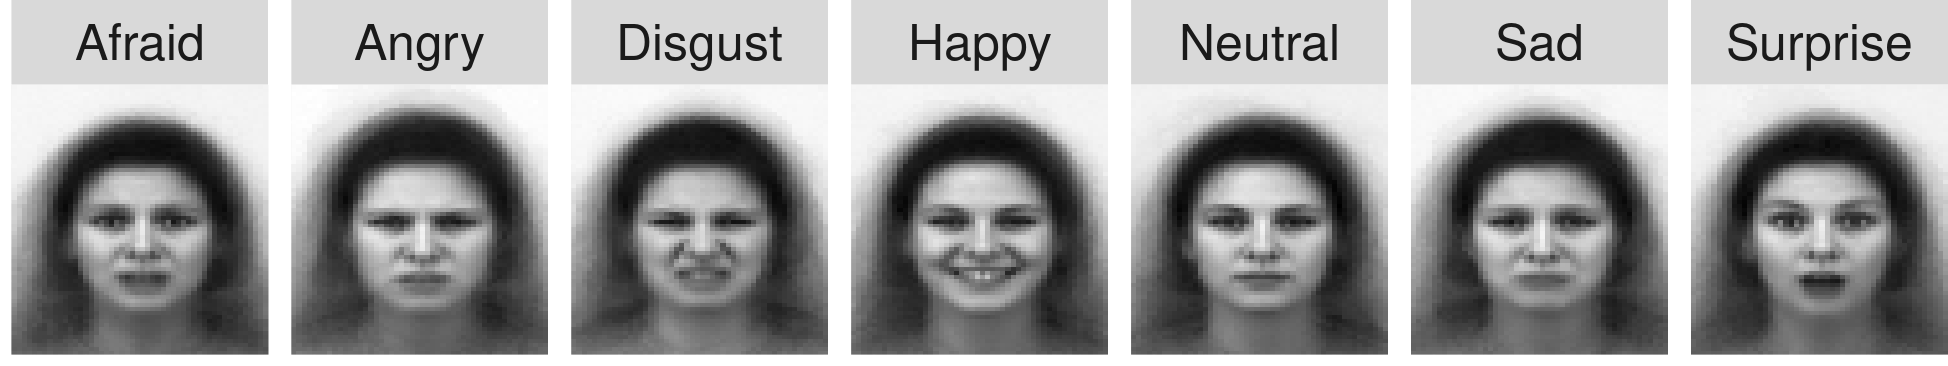
\includegraphics[height=4.0cm,width=\textwidth]{figure/mean_emotions.png}
%     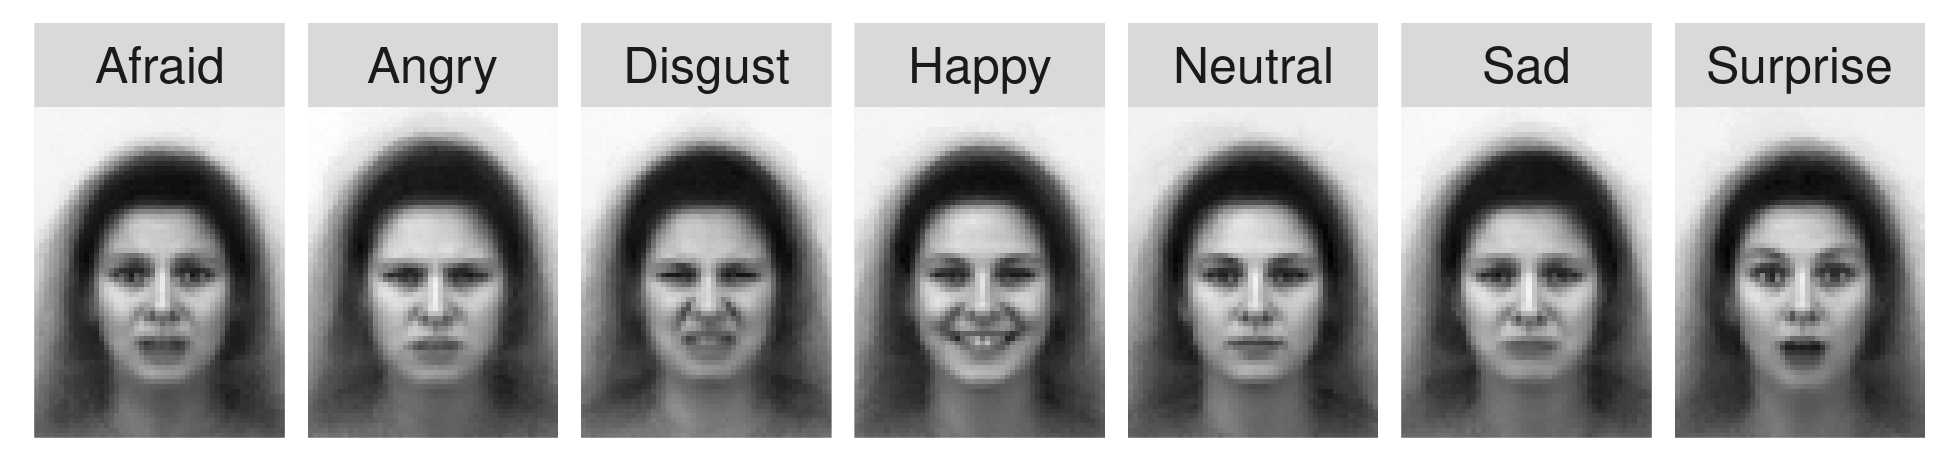
\includegraphics[height=5.0cm,width=\textwidth]{figure/mean_emotions_2rows.png}
%     \caption{}
%     \label{fig:faces-mean}
%     %Average Faces for Each Emotion
%     \end{subfigure}%
%   }\vfill
%   \hbox{%
%     \begin{subfigure}{.48\textwidth}
%     \centering
%     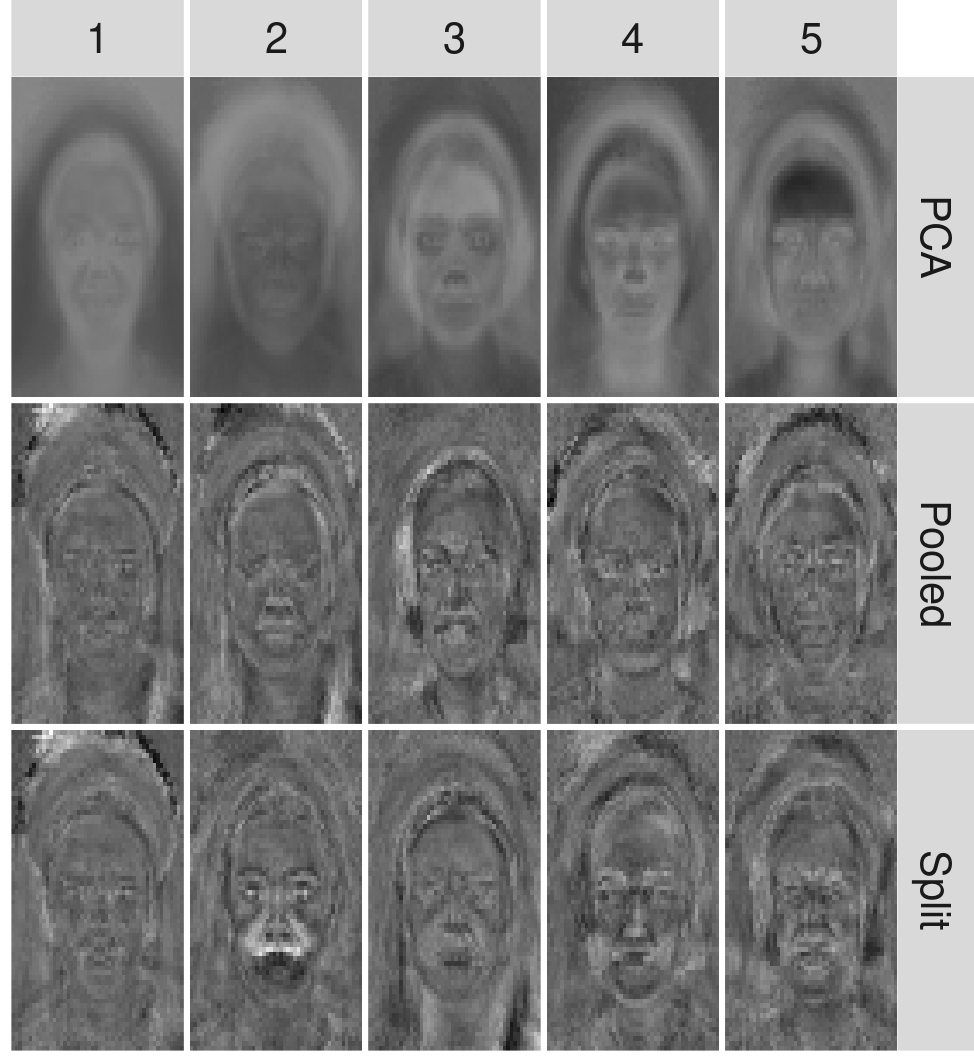
\includegraphics[height=8.0cm,width=\textwidth]{figure/all_Afraid_removed.png}
%     \caption{}
%     \label{fig:faces-eigenfaces}
%     %Top 5 Eigenfaces of Female Emotions by found by PCA, UCA with a pooled background, and UCA with backgrounds split
%     %\caption{Top five eigenfaces of Female Actors from KDEF \cite{Calvo2008}}
%     \end{subfigure}%
%   }\cr
% }
% \caption{
%   Results of analysis of KDEF faces. (a) Faces projected onto the first two components found by PCA, UCA with a pooled background, and UCA using multiple backgrounds. (b) Each emotion averaged over all female actors. (c) Top 5 eigenfaces of female emotions produced by different analyses.}
% \end{figure}

%\textbf{The faces in (b) look too squashed. Can you come up with a different arrangement of the subfigures? Also since some of the colors in the PCA are too similar, I had another idea, do you think we can do shapes as well? So like the ``bad'' emotions (anger, digust, etc.) get different shapes?}
% Solution: make PCA faces in (b) two rows.
% Rebuttal on PCA plot, can we leave it? it's supposed to look messy cause it's PCA

\begin{figure}
    \begin{subfigure}{\linewidth}
    \centering
    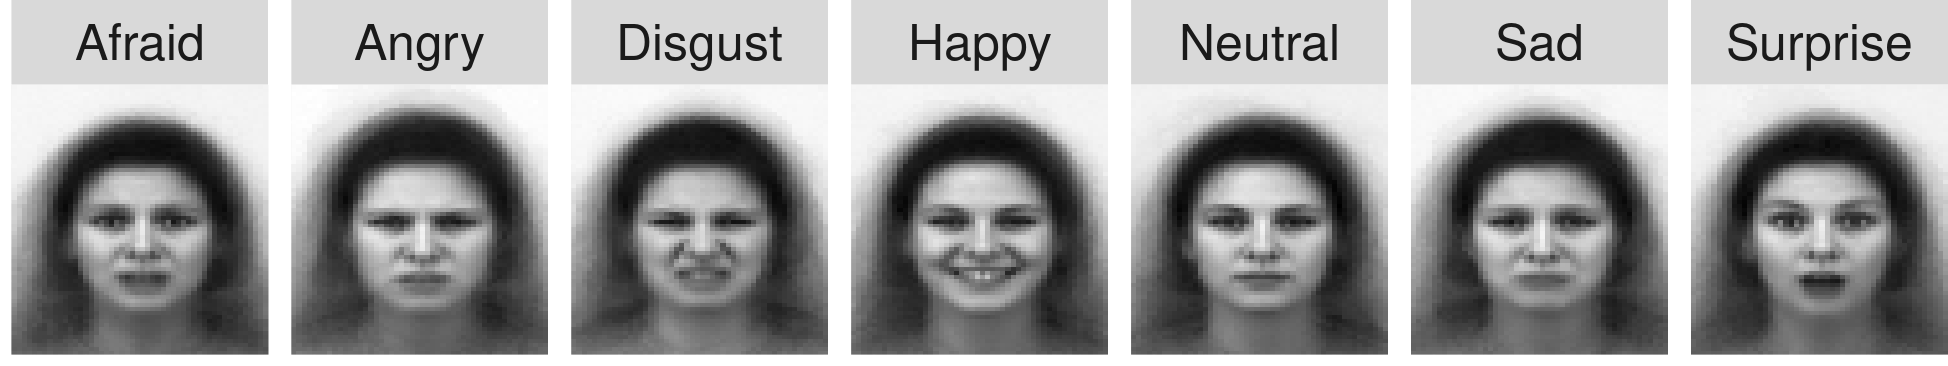
\includegraphics[height=3.0cm,width=\textwidth]{figure/mean_emotions.png}
    \caption{}
    \label{fig:faces-mean}
    %Average Faces for Each Emotion
    \end{subfigure}\\[1ex]
    \begin{subfigure}{.49\linewidth}
    \centering
    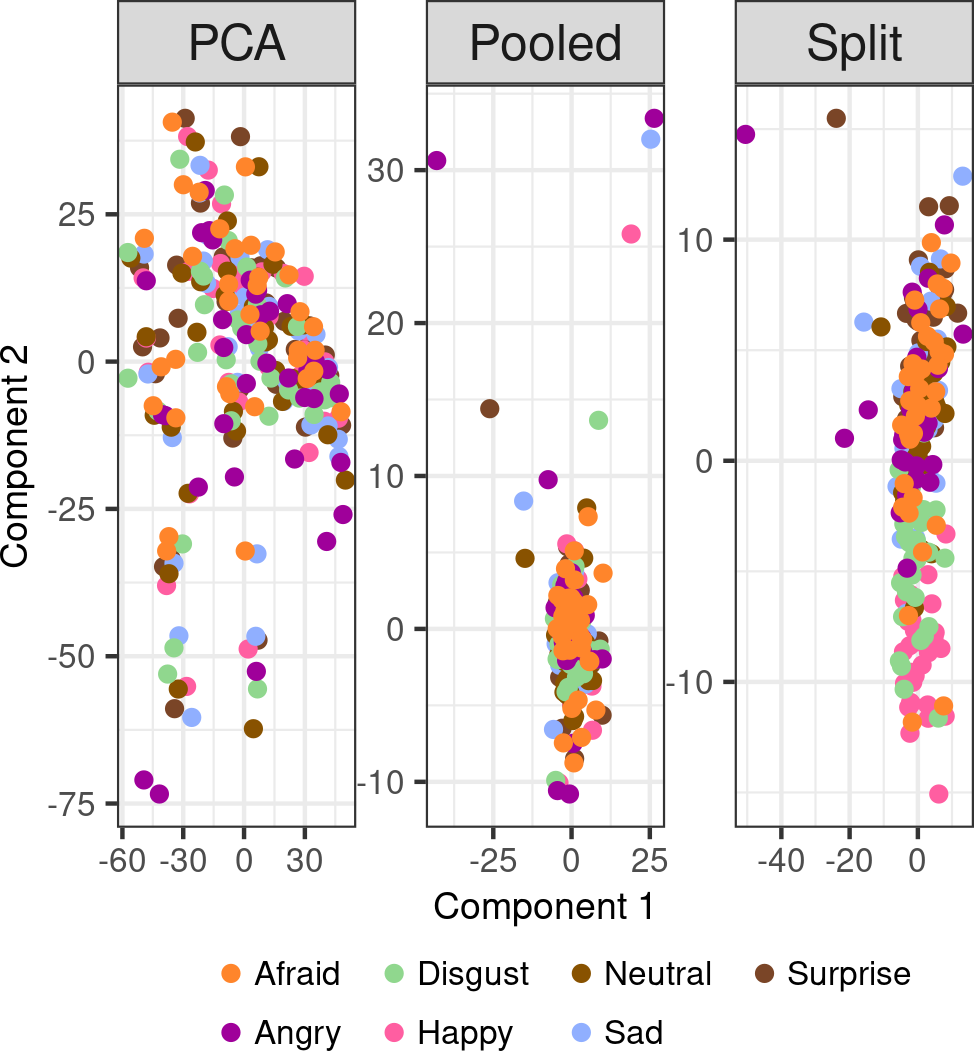
\includegraphics[height = 9.0cm,width=\textwidth]{figure/Afraid_projected_1_2_removed.png}
    \caption{}
    \label{fig:faces-projected}
    \end{subfigure}
    \begin{subfigure}{.49\linewidth}
    \centering
    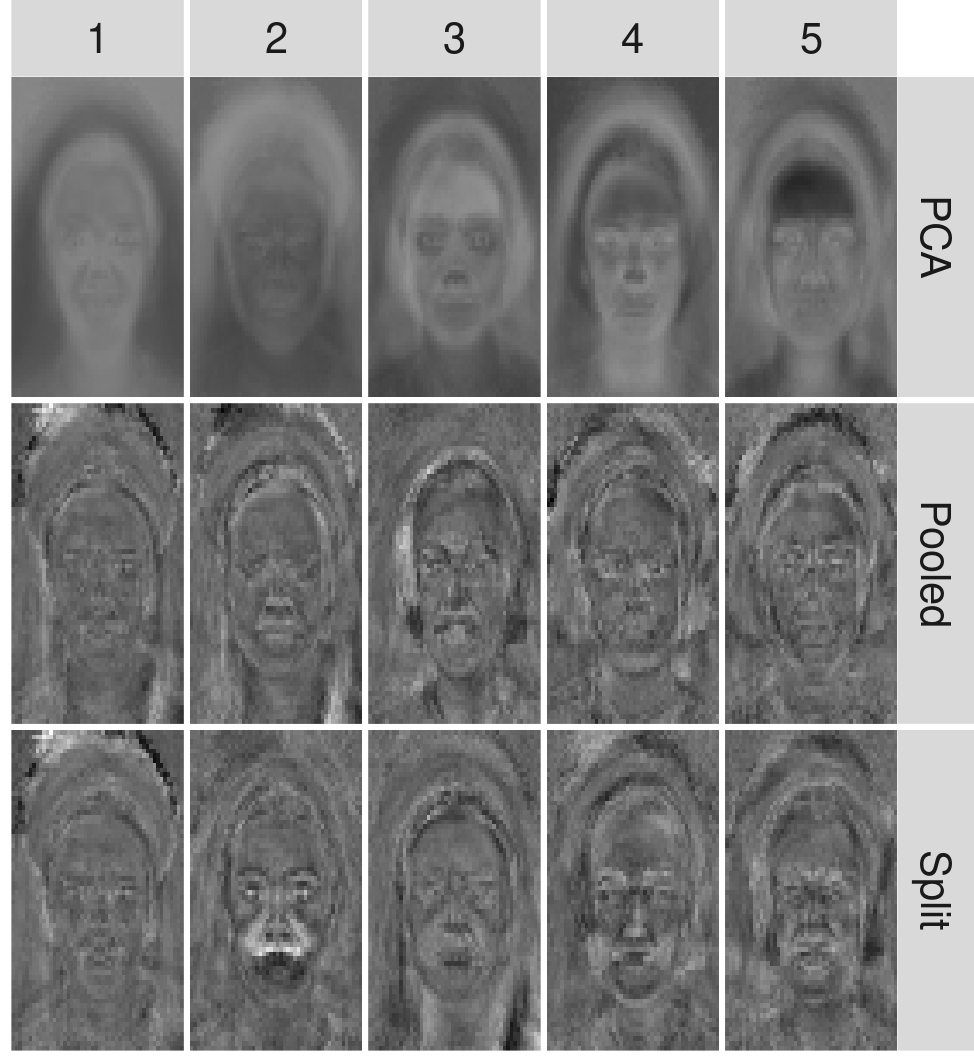
\includegraphics[height = 9.0cm,width=\textwidth]{figure/all_Afraid_removed.png}
    \caption{}
   \label{fig:faces-eigenfaces}
    \end{subfigure}
\caption{Results of analysis of KDEF faces.  (a) Each emotion averaged over all female actors. (b) Faces projected onto the first two components found by PCA, UCA with a pooled background, and UCA using multiple backgrounds. (c) Top 5 eigenfaces of female emotions produced by different analyses.}
\end{figure}

Figure \ref{fig:faces-projected} projects the target data onto the first two directions of variation calculated using each method. The emotions are entirely intermixed when projected onto components produced by PCA and by UCA using a single pooled background. In contrast, the emotions are much more separable when using UCA with multiple separate backgrounds. In particular, ``afraid'' faces are very separate from the ``disgust'' and ``happy'' faces. This indicates that UCA with multiple backgrounds can identify patterns of variation that can distinguish ``afraid'' from the other emotions.

Figure \ref{fig:faces-eigenfaces} shows visualizes the top five directions of variation produced by each method as faces. These are called eigenfaces, and this visualization technique is useful for interpreting the top components as facial features \cite{turk1991eigenfaces}. PCA eigenfaces generally represent features common to all the emotions. UCA eigenfaces using a pooled background seem to highlight the eyebrows and upper lips, though it is difficult to discern. On the other hand, eigenfaces produced using UCA using multiple separate backgrounds highlight eyebrows, eyes, nostrils, and nasolabial folds. These are especially clear in the second eigenface and accord with intuition about which features would likely be most useful in distinguishing ``afraid'' from other emotions.



% We see that in Figure \ref{fig:faces-mean}, which shows the mean face of each emotion, that the afraid emotion is characterized by eyebrows raised, eyes widened, nostrils opened, and mouth ajar. Features of afraid are most similar to that of surprise, where they differ only on height of eyebrows, nostril size, and nasolabial folds.

%concluding sentence

% \begin{figure}[!ht]
%   \label{fig:Diff_faces}
%   \centering
%   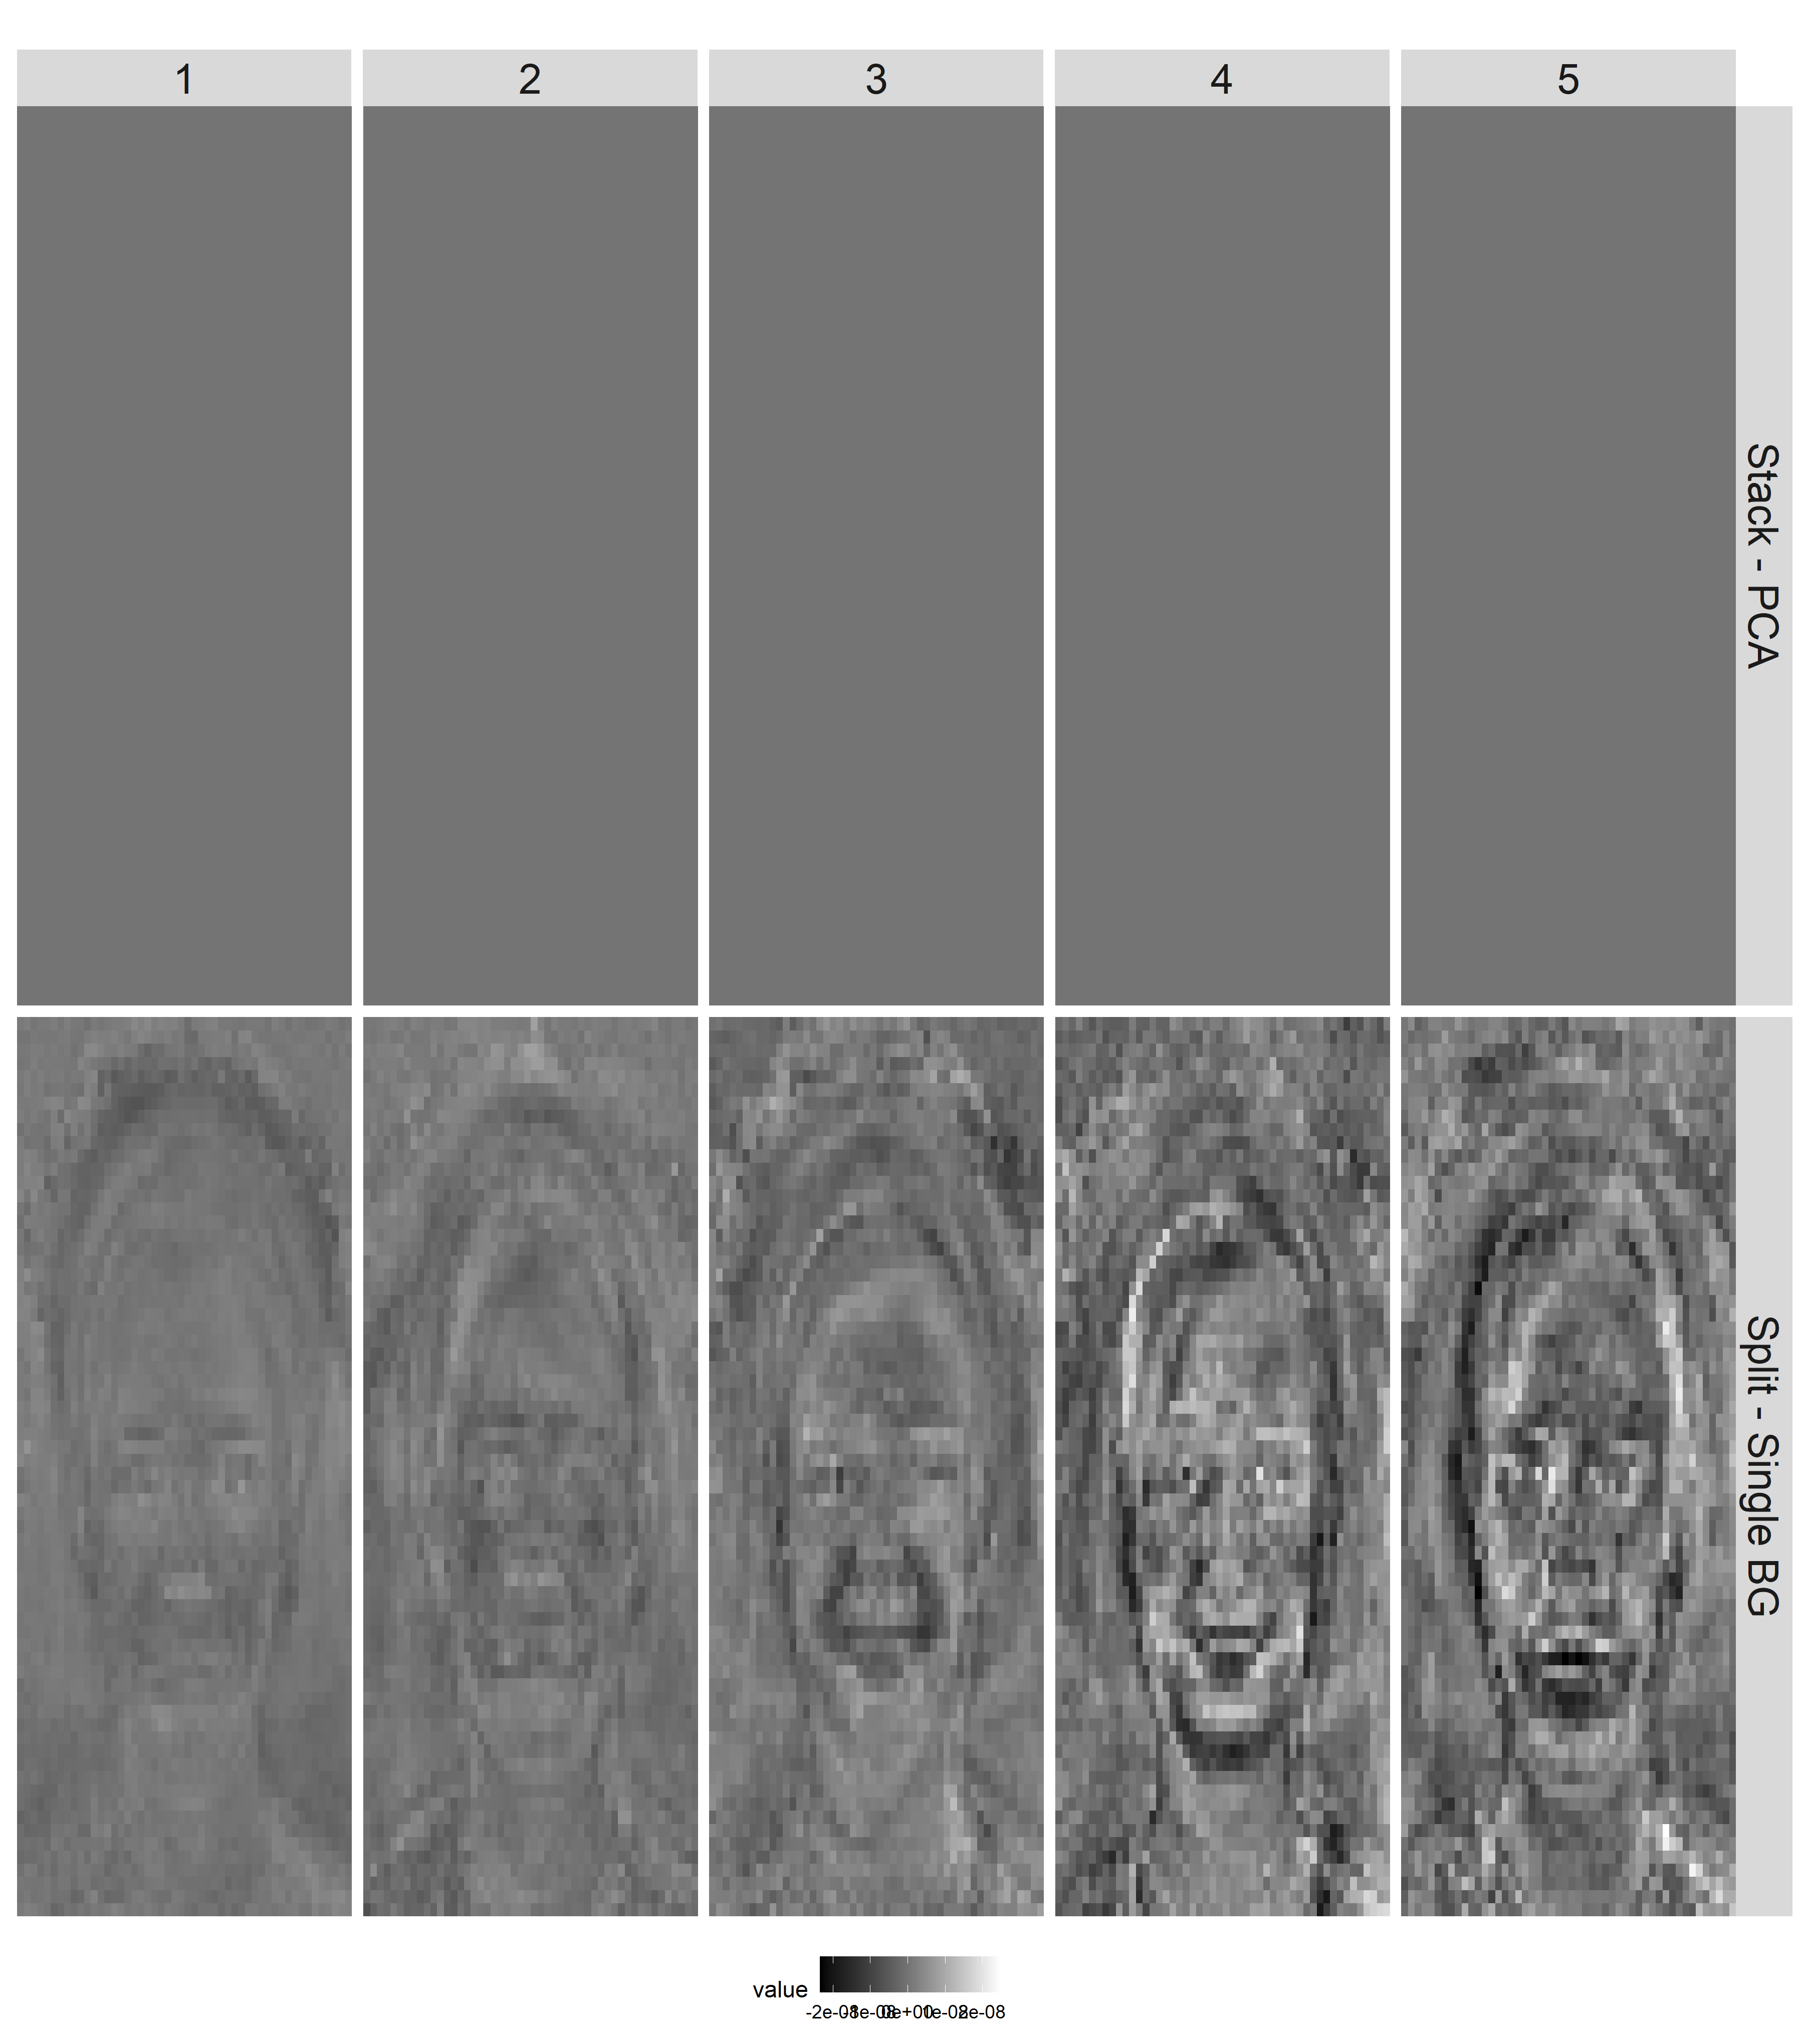
\includegraphics[width = 0.8\textwidth,height = 9cm]{figure/Happy_Neutral_Diff.png}
%   \caption{Eigenface difference images. Top row shows the difference between the eigenfaces produced by using a background of stacking neutral and neutral-inverse practice images, and PCA (no background image). The difference demonstrates that stacking multiple background datasets may lead to background data that is uninformative relative to the target, leading to features no different than PCA.  In contrast, when using UCA with two backgrounds where one background is uninformative (neutral practice and neutral-inverse faces as background), we get similar results to the single background (using only neutral practice faces) results}
% \end{figure}


% \subsection{MNIST}
% We use the numerical image data from MNIST \cite{MNIST} data to further illustrate the advantages of using multiple backgrounds as compared to a single background. This data contains 60,000 labeled training points and 10,000 labeled testing points of digits '0' through '9'.  In this example, we focus specifically on the numbers '4' and '9', which are among the most frequently confused numerical pairs.
% We compared PCA and UCA on the testing images of '4' and '9' under 4 scenarios: using only training images of '4', only training images of '9', combining training images of '4' and '9' via stacking, and utilizing training images of '4' and '9' separately (splitting).  This analysis shows us how the testing images of '4' and '9' load on the directions of maximal variation unseen in the background training images.

% The results of the rotated testing points of '4' and '9' using the first two components of PCA and UCA are seen in figure \ref{fig:MNIST}. It is clear that from the first two components, PCA has difficulty discerning differences between '4' and '9'. When using either '4' or '9' from the training data, the respective variability in the testing data is reduced. To reduce variability of both '4' and '9' in the testing data using the cPCA framework, we stack both the '4' and '9' training data together. However, after stacking, the rotated testing data of '4' and '9' overlap much more significantly than using either one individually, likely due to signal washout when constructing the joint background covariance matrix.  This effect is largely avoided when we treat '4' and '9' separate and construct separate covariance matrices with the training images: the testing points are more separable than using only the '4' background training data, only the '9' background training data, and stacking the '4' and '9' training data to construct a joint training covariance matrix.


% \begin{figure}[H]
%   \label{fig:MNIST}
%   \centering
%   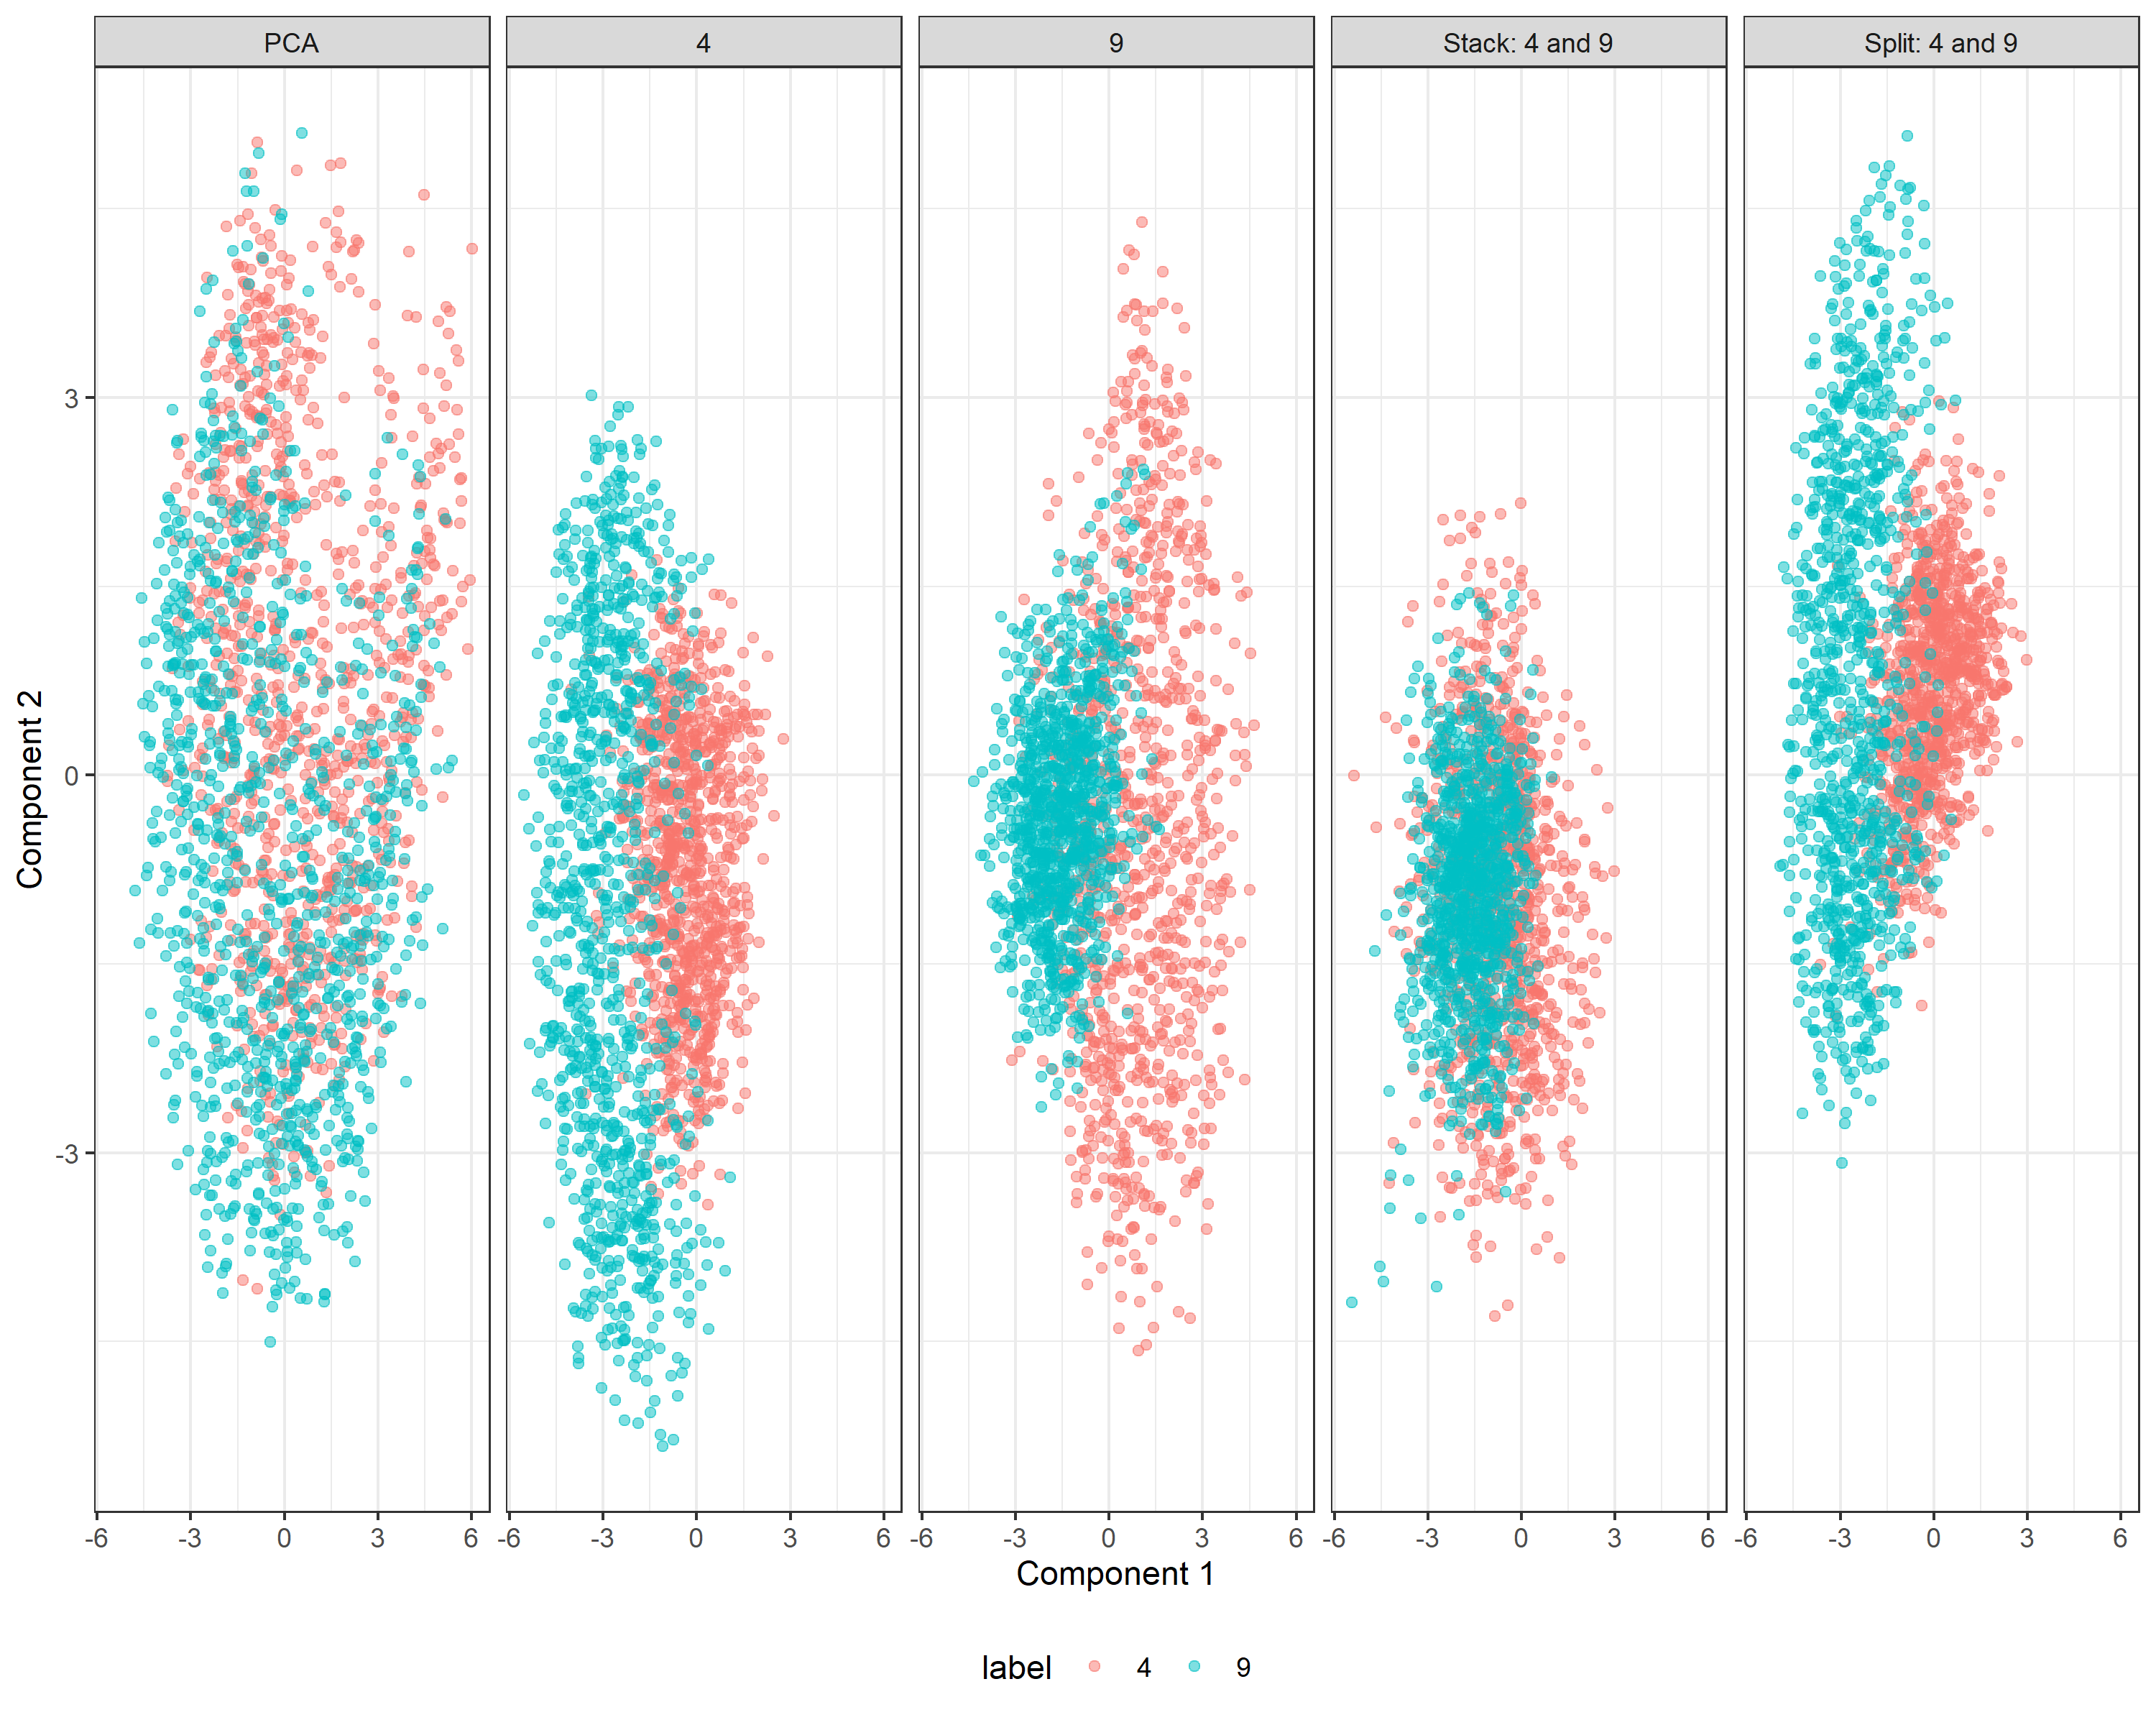
\includegraphics[width = 1.1\textwidth]{figure/MNIST_4_9_Stack_Split.png}
%   \caption{MNIST Data  \cite{MNIST} on the numbers '4' and '9', two commonly confused numerical values.  The target data consists of '4' and '9' from the testing portion of the MNIST data.  The background data (panel label in parenthesis) consists of nothing (PCA), only the labels '4' (4), only the labels '9' (9), both the labels '4' and '9' stacked as if it came from the same label group (Stack: 4 and 9), and the labels '4' and '9' if they were treated as separate backgrounds (Split: 4 and 9).  
%   The numbers '4' and '9' are not easily separable using PCA. Better separability is achieved when either '4' or '9' training data is used in the background.  }	
% \end{figure}

\section{Discussion}
In many data analytics settings, we are interested in removing uninteresting variation that contaminate the data of interest.
Here we proposed UCA, a tuning-free contrastive learning method that simplifies cPCA while also substantially improving it by accommodating multiple background datasets. We demonstrate UCA's usefulness and superiority in several examples. % To do this, we first solved the tuning parameter problem which plague current methods. UCA does not require user input in selecting the best contrastive parameter; rather it works by maximizing the target data variability subject to keeping the variability in each background small using weak duality of Lagrangians. 
% Moreover, we reformulate the contrastive problem to avoid creating several $p \times p$ covariance matrices, enabling us to perform contrastive analysis in high-dimensions.
We showed in analyses of mouse proteomics data and facial image data that UCA performs as well as cPCA when used with a single background dataset but can have dramatically better performance when used with multiple separate backgrounds.% is consistent with existing methods in the easily separable case within the mouse proteomics data. We then present a less separable case with the same mouse proteomics data, in which cPCA and cPCA++ fail to do an adequate job in separating Down Syndrome and control mice for any choice of tuning parameter, where applicable.
% We show that simply stacking individual background datasets can leverage multiple backgrounds to improve the single background separation between Down Syndrome and control mice.
% However, using the multiple background framework provided by UCA achieves even better results than stacking individual background datasets. 
% Lastly, we demonstrate that under the split framework unique to UCA, we can better separate each emotional face in the final session using the first two components, which cannot be accomplished with pooling multiple background data.  Other face combinations show either similar or better separation when treating backgrounds separately, rather than stacking them to form a joint covariance matrix.
% We hope that by providing a scalable, tuning-free, multibackground solution to the contrastive problem, UCA will play a pivotal role in isolating target variability in many scientific applications to come.
UCA is computationally fast and easily extensible to high-dimensional data because it does not require constructing nor storing a large covariance matrices (see Methods). Further, no additional post-hoc clustering method is necessary to choose the appropriate tuning parameter.

Like cPCA, the choice of background(s) still play a pivotal role in the directions found by UCA.
For background data that is already accounted for by other background data, the algorithm will ignore similar information and only weigh additional new information. In the event of identical backgrounds, only one background will be considered.
This can be avoided apriori by stacking data from the same experiments and creating a joint background. 

While the goal of UCA is not always to find separability between groups, UCA emphasizes finding variation in the target data scarcely seen in the background data. Therefore switching background data to it's compliment may not result in the same target data separation. 
For example, if our target data consists of all facial emotions in section \ref{sec:faces}, and our background consisted of negative emotions (Afraid, Angry, Disgust, Sad), we hope to see less variability in negative emotions and preserve variability in non-negative emotions (Happy, Surprise, Neutral).
Conversely, using non-negative emotions as the background instead would preserve the variability in negative emotions, and decrease the variability in non-negative emotions. What is scarcely seen in one set of background changes in the complement, resulting in different directions of variation. 
For maximal data seperation, we recommend using groups with larger variation as the background(s).
% not sure how to massage this point into the discussion...seems out of place
%   - backgounds help identify features that are important in the background. Imagine separating black from white where black is background. not white is a feature unique to background as well as black.
We have released the code for UCA as an R package, along with documentation and examples exhibited in this paper. 

% \textbf{Conclusion seems too short, do you have anything else to add? What does the original cPCA paper have in their discussion?}
%
%%% This is the discussion section in cPCA. %%%%%%
% In many data science settings, we are interested in visualizing and exploring patterns that are enriched in one dataset relative to other data. We have presented cPCA as a general tool for performing such contrastive exploration, and we have illustrated its usefulness in a diverse range of applications. The main advantages of cPCA are its generality and ease of use. Computing a particular cPCA takes essentially the same amount of time as computing a regular PCA. This computational efficiency enables cPCA to be useful for interactive data exploration, where each operation should ideally be almost immediate. As such, any settings where PCA is applied on related datasets, cPCA can also be applied. In the Supplementary Note 3 and Supplementary Fig. 8, we show how cPCA can be kernelized to uncover nonlinear contrastive patterns in datasets.
% 
% The only free parameter of contrastive PCA is the contrast strength α. In our default algorithm, we developed an automatic scheme based on clusterings of subspaces for selecting the most informative values of α (see Methods). All of the experiments performed for this paper use the automatically generated α values, and we believe this default will be sufficient in many applications of cPCA. The user may also input specific values for α if more fine-grained exploration is desired.
% 
% cPCA, like regular PCA and other dimensionality reduction methods, does not give p-values or other statistical significance quantifications. The patterns discovered through cPCA need to be validated through hypothesis testing or additional analysis using relevant domain knowledge. We have released the code for cPCA as a python package along with documentation and examples.
%%%%%%%%%%%%%%%%%%%%%%%%%%%%%%%%%%%%%%%%%%%%%%%%%%%


% cPCA++ isn't all that impressive
% background data choice is still very important. mouse data with control background gave terrible results

\section{Method}

% changes alpha to lambda.\textbf{DO YOU WANT TO CALL THIS ALPHA OR LAMBDA? NEED TO STAY CONSISTENT BETWEEN FIGURES, FIGURE CAPTIONS, AND TEXT}
% \textbf{BE CONSISTENT WITH CAPITALIZATION, etc.} checked: Lagrang[e|ian] multiplier eigendecomposition algorithm 

\subsection{Contrastive principal components analysis}
We first briefly review cPCA \cite{Abid}. Let $A$ denoted the $p\times p$ sample covariance matrix constucted from target data $X_{n_x \times p}$ and $B$ denote the $p\times p$ sample background covariance constructed from background data $Y_{n_y \times p}$. For some parameter $\lambda$, cPCA seeks the eigenvectors, $v_\lambda \in \mathbb{R}^p$, which account for large variation in the target data $Y$ and small variation in the background data $X$ where $\|v\|_2 = 1$. Specifically:  
\[v_\lambda = \text{arg}\max_{v \in \mathbb{R}^p}{\left(v^TAv - \lambda v^TBv\right)} \mbox{ subject to } v^\top  v = 1 \]

For a given $\lambda$, the direction is simply the eigenvector of the weighted difference between covariance matrices where $v$ maximize the variation in $A$ while constraining variation in $B$.
The tuning parameter $\lambda$ measures how much to penalize the background data covariance. When $\lambda = 0$, background variation is not considered, therefore cPCA reduces to PCA. As $\lambda$ increases, the relative background variation becomes more dominant, causing $v_\lambda$ to focus on directions which minimize background variation rather than maximizing the target. For very large values of $\lambda$, $v_\lambda$ is equivalent to PCA after projecting the target data onto the nullspace of the background data.  The authors of cPCA suggested that $\lambda$ be chosen using spectral clustering via a parameter sweep of logarithmically spaced candidate values.

We can rewrite the cPCA problem as a Rayleigh quotient
\[v_\lambda = \text{arg}\max_{v \in \mathbb{R}^p}{\frac{v^T\left(A - \lambda B\right)v}{v^T I v}}\]

and observe that the variability in $X$ and $Y$ are measured relative to the identity matrix.

\subsection{cPCA++}
%\textbf{Why does cPCA++ enforce $v^\top B v = 1$? We should explain.} It's not enforced, but 
%\textbf{How is this possible? Need to explain. Basically we need to explain how cPCA++ works before we explain UCA.}
Salloum and Kuo  \cite{Salloum} arrived at a tuning free contrastive method, cPCA++, where they seek to maximize the ratio, rather than the difference, of the variance explained in the target to the variance explained in the background.
%motivated by image splicing localization, classifying whether a pixel belonged to the original image or an image splice. Using a generalized likelihood ratio test framework to test whether a pixel belonged to foreground or background, they arrived at a Rayleigh Quotient of target variation divided by background variation.
Using similar notation as above where $A$ denotes the target sample covariance matrix and $B$ denotes the background sample covariance matrix, cPCA++ seeks to maximize the Rayleigh quotient:
\[v = \text{arg}\max_{v\in \mathbb{R}^p} \frac{v^T A v}{v^T B v}\]
% Rather than maximize the difference between the covariance matrices, relative to the identity matrix, they chose to maximize the quadratic term of $A$ relative to $B$.
% If we define $\lambda_{\text{max}} = \max_{v\in \mathbb{R}^p} \frac{v^T A v}{v^T B v}$, the maximum of the Rayleigh quotient, we see that $\left(v^T B v\right) \lambda_{\text{max}} = v^T A v$. 
% Such vectors $v$ have identical directions to solving the following primal problem and differ only by a scaling constant, c:
% \[
% \max_{v \in \mathbb{R}^p} v^\top A v \mbox{ subject to } v^\top B v = c.
% \]
% where $c = 1$ is a common identifiability constraint.
While maximizing the relative variability between $A$ and $B$ is tuning free, the solution involves a matrix inversion, which may not be feasible in high-dimensional applications like genomics where the inverse may not exist. Furthermore, there is no clear path to extend this problem to multiple backgrounds.
For clarity, We rewrite the cPCA++ objective function to it's primal form\cite{ghojogh2019eigenvalue}:
\[\max_{v \in \mathbb{R}^p}{v^T A v}  \mbox{ subject to } v^T B v = 1\]


%If $B$ is rank deficient, a choice of $\epsilon$ may be added to the diagonal terms to induce regularization.
%which does not require iterating through candidate contrastive parameters. This method uses a matrix inversion of a $p \times p$ background covariance matrix, which may be rank deficient, requiring the addition of some $\epsilon > 0$ onto the diagonal. The addition of $\epsilon$ onto the diagonal of the background matrix induces regularization depending on the choice of $\epsilon$, making this approach not exactly without tuning parameters.

\subsection{Unique Component Analysis}
We introduce the Unique Component Analysis (UCA) framework which combines both cPCA and cPCA++ to objectively solve for the contrastive parameter, $\lambda$ and resulting directions of variation using lagrangians. UCA works by joining the constraints of $v^T v = 1$ from cPCA and $v^T Bv = 1$ from cPCA++. For a single background covariance matrix UCA solves the primal problem: 
% These constraints are motivated by similar identifiablity constraints in generalized eigenvalue problems, e.g. PCA where $Av = \lambda Iv$ enforces $v^T v = 1$, cPCA++ where $Av = \lambda B v$ which enforces $v^T Bv = 1$. % allowing the principal components to be identifiable.
% Constraining $v^T v = 1$ while $v^T Bv$ is unconstrained may result in eigenvectors that explain large amounts of variability in the target but also explain large amounts of variability in the background.
% However, constraining $v^T Bv = 1$ while leaving $v^T v$ unconstrained results in eigenvectors that are not norm 1 and explain near zero variability in the target. 
% UCA combines both of these constraints together and can be expressed as a primal optimization problem:
\begin{align}
  &\max_{v\in \mathbb{R}^p}{v^TAv} \label{eq:1} \\ \text{subject to }&\; v^{T}v=1,\;\; v^TBv \leq 1 \nonumber
\end{align}
Since our primal problem is quadratic, strong duality requires satisfying Slater's condition\cite{boyd2004convex} (See Appendix B1).
To achieve strong duality, we require the smallest eigenvalue of $B$ to be less than 1, $\lambda_{\min}\left(B\right) = \min_{v}\frac{v^T B v}{v^T v}< 1$.
This requirement follows naturally for covariance matrices formed from standardized data due to the ordering of eigenvalues and:
\[tr(B) = \sum_{i = 1}^{p} \lambda_i = n\]
implies $\lambda_{\min}(B)\leq 1$, with equality if $B = I_p$.
For covariance matrices formed from unstandardized data, our assumption is the same as $dim(B) < p$, the dimensionality of $B$ is smaller than $p$. 
% covariance matrix $B$ is positive semi-definite, thus for all $v$, $v^T B v \geq 0$, implying existance of $v$ such that $v^T B v \leq 1$. 
With strong duality, we solve \ref{eq:1} by maximizing the dual function, $g(\lambda)$ of the Lagrangians $\mathcal{L}$:
\begin{align}
    \max_{\lambda \geq 0}{g(\lambda)} &= \max_{\lambda \geq 0}{\max_{v\in \mathbb{R}^{P}}{\mathcal{L}}}\left(v,\lambda\right) \nonumber\\
                                        &= \max_{\lambda \geq 0}{\max_{v\in \mathbb{R}^{P}}{\left( v^TAv - \lambda\left(v^TBv - 1\right)\right)}} \nonumber\\
                                        &= \max_{\lambda \geq 0}{\max_{v\in \mathbb{R}^{P}}{\left(v^T\left(A - \lambda B\right)v + \lambda\right)}}\nonumber\\
                                        &= \max_{\lambda \geq 0}{\left(\lambda_{\text{max}}\left(A - \lambda B\right) + \lambda\right)} \nonumber\\
                                        &= \max_{\lambda \geq 0}{\left(v_{\lambda}^T\left(A - \lambda B\right) v_{\lambda}+ \lambda\right)} \label{eq:2}
\end{align}
where $\lambda$ is the Lagrange multiplier associated with the constraint $v^T Bv \leq 1$, $\lambda_{\max}(A - \lambda B)$ is the largest eigenvalue associated with $A - \lambda B$, and $v_{\lambda}$ is the corresponding eigenvector. Although the primal problem has two constraints, $v^T v = I$ is enforced through eigendecomposition when solving for the largest eigenvalue $\lambda_{\text{max}}$. % This is slightly different from cPCA++, where $v^{T}v$ is not necessarily orthonormal.

Since the dual function is concave and a solution necessarily exists, we maximize the dual function \eqref{eq:2} by taking the derivative with respect to $\lambda$ and set the derivative equal to zero: 

\begin{align}
    \frac{\partial}{\partial\lambda} g(\lambda) &= \frac{\partial}{\partial\lambda} \left(v_{\lambda}^T\left(A - \lambda B\right) v_{\lambda}+ \lambda\right)\nonumber \\ 
                                                &\Leftrightarrow \frac{\partial}{\partial\lambda}\left( -\lambda \left(v_{\lambda}^{T} Bv_{\lambda}\right) + \lambda \right) \nonumber\\
                                                &= 1-v_\lambda^{T}B v_{\lambda} = 0 \label{eq:3}
\end{align}

%\textbf{Also, it's not immediately clear where you used a eigendecomposition. An eigendecomposition is a factorization of a matrix $M = V \Sigma V^\top$, but I don't see a matrix factorization here. I think you can be more precise about what exactly you did.}
We use an iterative algorithm (L-BFGS-B) \cite{byrd1995limited} to search for Lagrange multiplier $\lambda$ such that the associated eigenvectors $v_\lambda$ satisfies equation \ref{eq:3}.
Due to strong duality, the resulting $v_\lambda$ also solves the primal problem.
We see that combining the two constraints allows us a natural way to solve for the contrastive parameter $\lambda$ in cPCA when only one background is used.
% \textbf{How do you know that this interation between $\lambda$ and $v_\lambda$ will converge, and if it converges, how do you know it will converge to a global rather than local optimum?}
% Similar to the constrastive parameter, the Lagrange multiplier can't be less than zero, and allows us to use box constrained optimization methods. 
% How do you know this converges? Can we rely on the concavity of the dual function to say that this is a global optimum since no duality gap?
% comment on uniquness or is this obvious?

%% is it worth mentioning if A, B are the same, lambda = 1? connections to likelihood ratio test?
%% For the special case when covariance matrices $A$ and $B$ are the same, the constraint forces $\lambda = 1$ because as $\lambda \rightarrow 1^-$, the largest eigenvalue approaches zero and for $\lambda \geq 1$, the largest eigenvalue is zero.

% \textbf{NO NEED TO SEPARATE SINGLE AND MULTIPLE BACKGROUNDS INTO TWO SECTIONS. MOTIVATE THE OPTIMIZATION PROBLEM FOR ONE BACKGROUND, THEN EXTEND TO MULTIPLE, THEN PROVIDE GENERAL ALGORITHM THAT WORKS FOR SINGLE OR MULTIPLE.}

Similarly, for multiple backgrounds, again let the $A$ be the target $p \times p$ covariance matrix and $ B_1, \ldots, B_m$ now be the $m$ background $p \times p$ covariance matrices constructed from a $n_y \times p$ dimensional Y data matrix and corresponding $(n_{x_1} \times p), \ldots, (n_{x_m}\times p)$ dimensional $X_1, \ldots, X_m$ background data matrices.
% One way to incorporate $m$ background would be to use the framework in the single background setting and stack multiple background datasets before calculate the background covariance matrix, creating a weighted average of the covariance matrices. This is sub-optimal since the background covariance matrix with the most samples may not accounts for the all the background noise, therefore potentially washing out background noise from the other smaller background datasets. 
% A more natural way to incorporate $m$ background datasets in a more generalized framework would be to append the background matrices like so:
% \[\max_{v\in \mathbb{R}^p}{v^T\left(A - \sum^{m}_{j=1}{\lambda_jB_j}\right)v}\]
% However, a parameter sweep for each $\lambda_j$ corresponding to background data $B_j$ would be computationally expensive.
% We can easily extend our single background covariance method to address the $m$ background covariance scenario by adding additional constraints to Lagrangian,
We add additional constraints $ v^TB_jv\leq 1$ to our optimization problem for each background $j = 1, \ldots, m$. Specifically, for multiple backgrounds, the primal problem becomes
\begin{align}
  &\max_{v\in \mathbb{R}^p}{v^TAv} \label{eq:4}\\ 
  \text{subject to }&\; v^{T}v=1,\;\; v^TB_1 v \leq 1, \ldots, v^T B_m v\leq 1 \nonumber
\end{align}
Maximizing the corresponding dual function $g(\lambda_1, \ldots, \lambda_m)$:
\begin{align}
    \max_{\lambda_1,\ldots,\lambda_m \geq 0}{g(\lambda_1, \ldots, \lambda_m)} &= \max_{\lambda_1,\ldots,\lambda_m \geq 0}{\max_{v\in \mathbb{R}^{P}}{\mathcal{L}\left(v, \lambda_1, \ldots, \lambda_m\right)}} \nonumber \\
  %&=\max_{\lambda_1,\ldots,\lambda_m \geq 0}{\max_{v\in \mathbb{R}^{P}}{\left(v^TAv - \lambda_1\left(v^TB_1v - 1\right)-\ldots -\lambda_m\left(v^TB_mv - 1\right)\right)}}\nonumber \\
                                                                                                                                &=\max_{\lambda_1,\ldots,\lambda_m \geq 0}{\max_{v\in \mathbb{R}^{P}}{\left(v^T\left(A - \sum^{m}_{j = 1}{\lambda_j B_j}\right)v + \sum^{m}_{j=1}{\lambda_j}\right)}} \nonumber\\
                                                                                                                                &=\max_{\lambda_1,\ldots,\lambda_m \geq 0}{\left(\lambda_{\text{max}}\left(A - \sum^{m}_{j = 1}{\lambda_j B_j}\right) + \sum^{m}_{j=1}{\lambda_j}\right)} \label{eq:5}
\end{align}

For background $j \in 1,...,m$, we can solve for the $j$th Lagrange multiplier in equation \ref{eq:5} similarly by taking the partial derivative and setting to zero:
\begin{align}
    \frac{\partial}{\partial \lambda_j}\left(\lambda_{\text{max}}\left(A - \sum^{m}_{j = 1}{\lambda_j B_j}\right) + \sum^{m}_{j=1}{\lambda_j}\right)&=\frac{\partial}{\partial \lambda_j}v_{\lambda}^T\left(A - \sum^{m}_{j = 1}{\lambda_j B_j}\right)v_{\lambda} + \sum^{m}_{j=1}{\lambda_j}\nonumber\\
                                                                                                                                                    &\Leftrightarrow \frac{\partial}{\partial \lambda_j}\left(v_{\lambda}^T\left(A - \lambda_j B_j \right)v_{\lambda}+\lambda_j\right)\nonumber \\ 
                                                                                                                        &\Leftrightarrow \frac{\partial}{\partial \lambda_j}\left(-\lambda_j v_{\lambda}^T  B_j v_{\lambda} +\lambda_j \right)\nonumber \\ 
                                                                                                                        &= 1-v_{\lambda_j}^{T}B_j v_{\lambda_j} = 0 \label{eq:6}
\end{align}
%\textbf{Again, how do you know that this coordinate descent algorithm will converge to a global optimum?}
To solve this multiple background dataset problem we propose a coordinate descent algorithm that utilizes the single background dataset L-BFGS-B \cite{byrd1995limited} algorithm iteratively. 
For $m$ background datasets, on the $q^{th}$ iteration, let $A_{(j)}^*$ be the variation in $A$ after excluding background variation that is not $B_j$:
\[A_{(j)}^{*} = A - \sum_{ i = 1 }^{j-1}\lambda_{i}^{(q+1)}B_i - \sum_{i =j+1}^{m}\lambda_{i}^{(q)}B_i \] \
to solve for $j^{th}$ of the $m$ Lagrange multipliers, we use Algorithm \ref{alg:uca-multiple}.

% add input and output into algorithm
\begin{algorithm}[ht]
  \caption{coordinate descent algorithm}
  \label{alg:uca-multiple}
  \textbf{Inputs: } $m$ centered background data $X_1,\ldots, X_m $, centered Target data $Y$, $k$ number of components\;
  Initialize $\lambda_{1}^{(0)}, \ldots,\lambda_{m}^{(0)} $, $\epsilon$\;
  Compute the emperical covariance matrices:
  \[A = \frac{1}{n_y}Y^TY,\;\; B_1 = \frac{1}{n_{x_1}}X_1^TX_1,\;\ldots, B_m = \frac{1}{n_{x_m}}X_m^TX_m\; \]
  \While{$l^{(q+1)} - l^{(q)} > \epsilon$}{
    \For{ $j = 1:m$}{
      Solve for $\lambda_j^{(q+1)}$ via L-BFGS-B, corresponding to the largest eigenvalue of \[C_{\lambda_j} = A_{(j)}^{*} - \lambda_j^{(q+1)}B_j\] \
      % with corresponding eigenvector, $v_{\lambda_{j}^{(q+1)}}$, satisfying:
      % \[1 -v_{\lambda_{j}^{(q+1)}}^{T} B_j v_{\lambda_{j}^{(q+1)}} = 0\]
    }
    After iterating through $m$ Lagrange multipliers, calculate value of Lagrangian
    \[l^{(q+1)} = \lambda_{max}\left(A-\sum^{m}_{j=1}\lambda_{j}^{(q+1)}B_j\right)+ \sum^{m}_{j=1}\lambda_{j}^{(q+1)}\]\
  }
  Compute \[C_{\lambda_1, \ldots, \lambda_m} = A - \sum^{m}_{j = 1}{\lambda_j B_j}\]
  Find $V_k\in \mathbb{R}^k$, spanned by the top $k$ eigenvectors of $C_{\lambda_1, \ldots, \lambda_k}$\;
  \textbf{Return: } $V_k$
\end{algorithm}


% The advantage to the Lagrangian method in the multiple background setting is that rather than constructing an aggregated covariance matrix by stacking data, which arbitrarily weighs covariance matrices by their sample size, our method objectively constructs weights which satisfy the constraint $ v^TB_jv\leq 1$ for each $m$ background covariance matrix. If multiple backgrounds contain the same information, constructing the covariance matrix by stacking data will change the covariance by a factor less than 1, e.g. for two backgrounds, the covariance changes by $\frac{2}{2n - 1}$.  If only one covariance matrix will constrain the Lagrangian, the corresponding Lagrange multiplier will be non-zero and Lagrange multipliers corresponding to all other redundant constraints on the Lagrangian are set to zero.  

\subsection{Extension to High Dimensional Data:}

\begin{figure}[!ht]
  \centering
  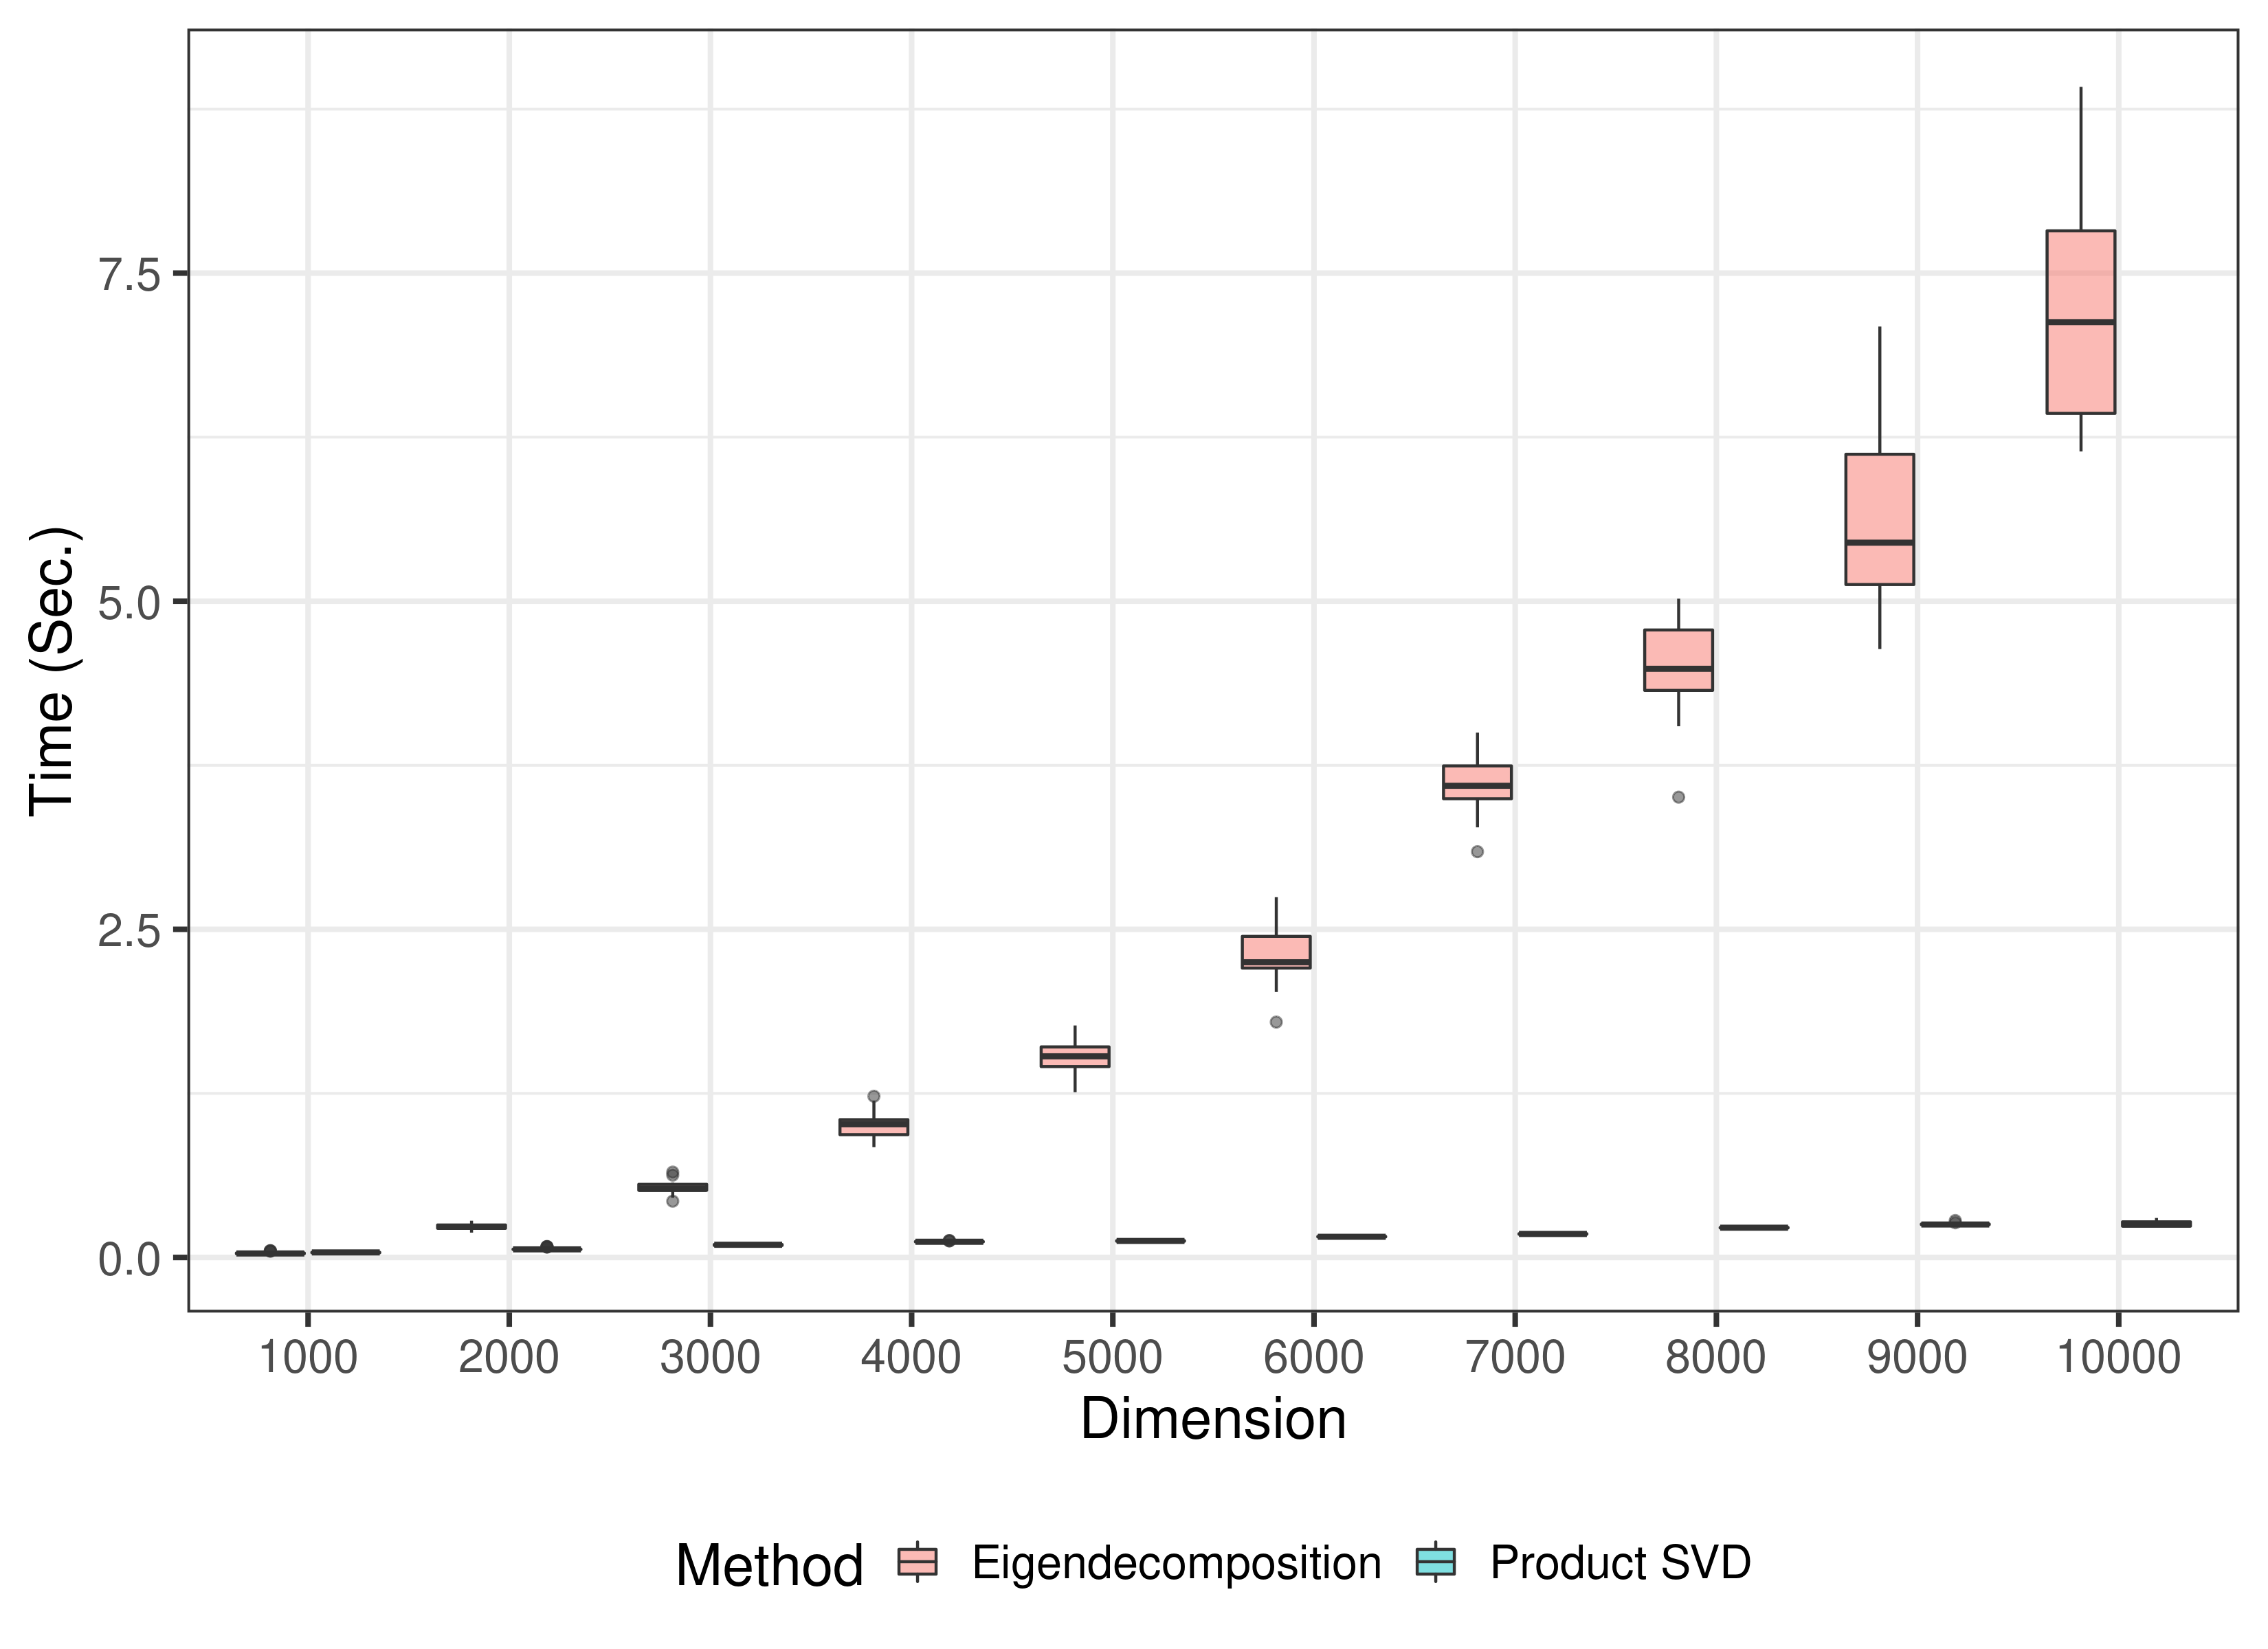
\includegraphics[width = 0.8\textwidth]{figure/final_perf.png}
  \caption{UCA and cPCA implementation using Product SVD vs. eigendecomposition for high-dimensional data: 25 random $100 \times p $ target and background matrices are generated from a standard normal distribution and where $p$, the dimension varied from 1,000 to 10,000 in steps of 1,000. Box plots of time (in seconds) is plotted for both eigendecomposition and the product SVD method. For small $p$, there is a negligible difference between the methods. However, as dimension $p$ increases, the Product SVD is significantly faster.}
  \label{fig:computational_perf}
\end{figure}

% \textbf{First need to explain what the problem is when we have high-dimensional data. Actually first need to explain what high-dimensional data means.}
Under the high-dimensional situation, where the number of variables $p$ far exceeds the number of samples $n$, constructing the covariance matrix and using eigendecomposition to find the top eigenvectors becomes computationally expensive. To avoid the intermediatary of creating and storing a large $p \times p$ covariance matrix, singular-value decomposition (SVD) of the data matrix is frequently used to find the top eigenvalue/eigenvectors of its covariance.
To extend our method to high-dimensional data, we analogously avoid the traditional eigendecomposition method of finding eigenvalue/eigenvectors of the covariance matrix that current methods employ.
We introduce the Product SVD method to exploit the structure of how the contrastive covariance matrices are formed and employ SVD of a product of matrices to quickly find our top eigenvalue.  Breaking the problem down in this way considerably speeds up our L-BFGS-B algorithm, and allows us to run UCA even in the high-dimensional setting.

For a single background, let the $p \times p$ covariance matrices $A$ be the target covariance matrix and $B$ be the background covariance matrix. $A$ and $B$ are formed from corresponding centered $n_y \times p$ target data matrix $Y$,   and centered $n_x \times p$ background data matrix $X$.  We can write the difference of the covariance matrices $A - \lambda B$ as a product of a $p \times (n_y + n_x)$ dimensional left matrix , $L$, and a $(n_y + n_x) \times p$ dimensional right matrix, $R$ as seen in equation \ref{eq:7}:
\begin{align}
  C_\lambda &= A - \lambda B \nonumber\\
            &=\frac{1}{n_y}Y^TY -\frac{\lambda}{n_x} X^T X\nonumber \\
            &=  \underbrace{\left[ \frac{1}{\sqrt{n_{y}}}Y^T, - \frac{\lambda}{\sqrt{n_{x}}} X^T\right]}_{L}\underbrace{\begin{bmatrix*} \frac{1}{\sqrt{n_{y}}}Y \\ \frac{1}{\sqrt{n_{x}}}X \\ \end{bmatrix*}}_{R} \label{eq:7}
\end{align}
With this formulation, we can follow the steps in Golub et al.  \cite{Golub}, and find the singular values and vectors of $C_\lambda$ using a sequence of SVD and QR decompositions operating on the left and right matrices. Since singular values and eigenvalues coincide in square matrices, we use the singular vectors, $U$, to find the largest eigenvalues by sorting the diagonal of $ULRU^T$.  
We describe the Product SVD Method in algorithm \ref{algo:product-svd}, which can directly replace the more computationally expensive eigendecomposition in high dimensions.

\begin{algorithm}[ht]
  \caption{Product SVD Method to calculate the largest Eigenvalue of $C_\lambda$}
  \label{algo:product-svd}
  \SetAlgoLined
  \textbf{Input:} Centered background matrix $X$, centered target matrix $Y$, and $\lambda$\;
  \nl Construct 
  $  L = \left[ \frac{1}{\sqrt{n_{y}}}Y^T, - \frac{\lambda}{\sqrt{n_{x}}} X^T\right],\;
  R = \begin{bmatrix*} \frac{1}{\sqrt{n_{y}}}Y \\ \frac{1}{\sqrt{n_{x}}}X \\ \end{bmatrix*} $\;
  \nl  SVD the right matrix, $R = U_R S_R V^T_R$ \;
  \nl  QR decompose $LU_R$ into  $Q_{LU_R}R_{LU_R}$ \;
  \nl  SVD the product of $R_{LU_R}$ (step 3) and $S_R$ (step 2), $R_{LU_R}S_{R} = EDF^T$ \;
  \nl  The singular vectors of $C_\lambda$ is the product of $Q$ (step 3) and $E$ (step 4), $U_{C_\lambda} = Q_{LU_R}E$ \;
  \nl  Find the largest eigenvalues of $C_\lambda$ by sorting the diagonal of $D_{C_\lambda}$, where $D_{C_\lambda} = U_{C_\lambda} C_\lambda U_{C_\lambda}^T$ \;
  \textbf{Output:} $\lambda_{\text{max}}\left( C_\lambda \right)$ 
\end{algorithm}

Similarly, for multiple backgrounds, again let the $A$ be the target $p \times p$ covariance matrix and $ B_1, \ldots, B_m$ be the $m$ background $p \times p$ covariance matrices constructed from a $n_y \times p$ dimensional Y data matrix and corresponding $(n_{x_1} \times p), \ldots, (n_{x_m}\times p)$ dimensional $X_1, \ldots X_m$ background data matrices.

We can construct $C_{\lambda_1, \ldots, \lambda_m} = A - \sum^{m}_{j=1}\lambda_jB_j$ analogously by appending the additional datasets to the left and right matrices:
\begin{align}
  C_{\lambda_1, \ldots, \lambda_m}&= A - \sum^{m}_{j=1}\lambda_jB_j \nonumber \\
                                  &=\frac{1}{n_y}Y^{T}Y -\sum_{j=1}^{m}{\frac{\lambda_{j}}{n_{x_j}}X_{j}^TX_{j}} \nonumber\\
                                  &=  \underbrace{\left[\frac{1}{\sqrt{n_y}}Y^T, -\frac{\lambda_1}{\sqrt{n_{x_{1}}}} X^T_1, \ldots, -\frac{\lambda_m}{\sqrt{n_{x_{m}}}}X^T_m\right]}_{L} \underbrace{\begin{bmatrix} \frac{1}{\sqrt{n_{y}}}Y \\ \frac{1}{\sqrt{n_{x_{1}}}}X_1 \\ \vdots \\ \frac{1}{\sqrt{n_{x_{m}}}}X_m \end{bmatrix}}_{R} \label{eq:8}
\end{align}
Using the coordinate descent (algorithm \ref{alg:uca-multiple}) to solve for each $\lambda_j$ prescribed above, we can substitute the eigendecomposition of the covariance matrix, $C_{\lambda_{j}}$ with the Product SVD method (algorithm \ref{algo:product-svd}) using $L$ and $R$ defined in equation \ref{eq:8}.

The Product SVD method is advantageous in high-dimensions because it never explicitly operates on the entire $p \times p$ covariance matrix. Not only is our method more memory efficient, scaling with $n\times p$ bytes rather than $p^2$ bytes, but our method is also computationally more efficient at finding the largest eigenvalue/eigenvector as operating SVD and QR decomposition on either the left or right matrices is faster than directly operating eigendecomposition on the covariance matrix. In the single background scenario,  $\lambda$ only appears in $L$. Thus since, $R$ doesn't change, we can pre-compute the SVD of $R$, and only update $L$ when solving for $\lambda_{\text{max}}$.
Similarly, in the multi-background scenario, rather than modifying $A^*$ in the original coordinate descent algorithm, this method allows us to only modify the $j+1$ element of the left data matrix, $L$.
The SVD of the right matrix, $R$, only needs to be computed once in our coordinate descent. Furthermore, at each step within the coordinate descent only step 3 and 4, the SVD and QR, are computed, and are done on matrices with dimensions much smaller than $p \times p$.

To demonstrate the speed improvements of the Product SVD method compared to the current fastest implementations of eigendecomposition in high-dimensions, we conduct a simulation study with 25 sample $100 \times p$ target and background data matrices generated from a standard Normal distribution with $p$ varying from 1.000 to 10,000 in steps of 1,000. To ensure a fair comparison, we leverage C++ in both implementations using a custom RcppArmadillo \cite{rcpparmadillo} function for the Product SVD method and the RSpectra package (0.16-0) \cite{Rspectra} for the eigendecomposition method; RSpectra being a package designed for large-scale eigendecompositions based off the C++ Spectra library. We use the microbenchmark package \cite{microbenchmark} to ensure accurate timings. Our benchmark does not take into account the additional cost of forming the $p\times p$ covariance matrices, which would only exacerbate the difference between the two methods in real world applications.

Figure \ref{fig:computational_perf} show box plots of time (in seconds) versus the dimension, $p$, colored by method, summarizes the results of the simulation study. As dimension $p$ increases, the computational time of our Product SVD method increases much slower than the current eigendecomposition implementations. It should be mentioned that for $p < 1000$ the Product SVD method is slower due to overhead of additional computation on small matrices. In general, for low-dimensional settings where $n \geq p$, the Product SVD will be negligibly slower because of the additional QR, SVD, matrix products, and sort computations. 

% More concretely, an UCA analysis of a target $3400\times 3400$ dimensional covariance matrix with two backgrounds requires 88 MB of storage for each of the three covariance matrices formed, compared to 1.8 MB for each data matrix.  Assuming these matrices have all been pre-calculated, using a RSpectra implementation of eigendecomposition, UCA takes 93 seconds vs. 9 seconds with our method.

All computations in this paper were done with R 3.6.3 \cite{baseR} on an AMD Ryzen 1700X 3.7 gHz processor and 64GB 3000 mhz DDR4 RAM, utilizing the Intel MKL libraries. 

%\textbf{I think you should explicitly write out the URLs in addition to links, that's what I usually see people doing.}

% these subsections are just copies of cPCA paper...
% \subsection{Theoretical Guarantees}
% \subsection{Choosing Background Data}
\subsection{Code Availability}
We have released a R implementation of \href{https://github.com/rtud2/Residual-Dimension-Reduction}{https://github.com/rtud2/Residual-Dimension-Reduction}. We have implemented both Product SVD on the data matrix and eigendecomposition on the contrastive covariance matrix and allow the background to take either a single background or a list of backgrounds. The GitHub repository also includes R markdown and datasets that reproduce most of the figures in this paper and in the Supplementary.

\subsection{Data availability}
Datasets that have been used to evaluate UCA in this paper are publicly available from the authors of the original studies. The mouse proteomics data are available from the UC Irvine Machine Learning Repository \url{https://archive.ics.uci.edu/ml/datasets/Mice+Protein+Expression}\cite{Higuera} and the Karolinska Directed Emotional Faces (KDEF) are available from \url{https://www.kdef.se/}\cite{Calvo2008}.


\bibliographystyle{plain}
\bibliography{mybib}

 % \section{Appendix}
 % \begin{figure}[!ht]
 %   \centering
 %   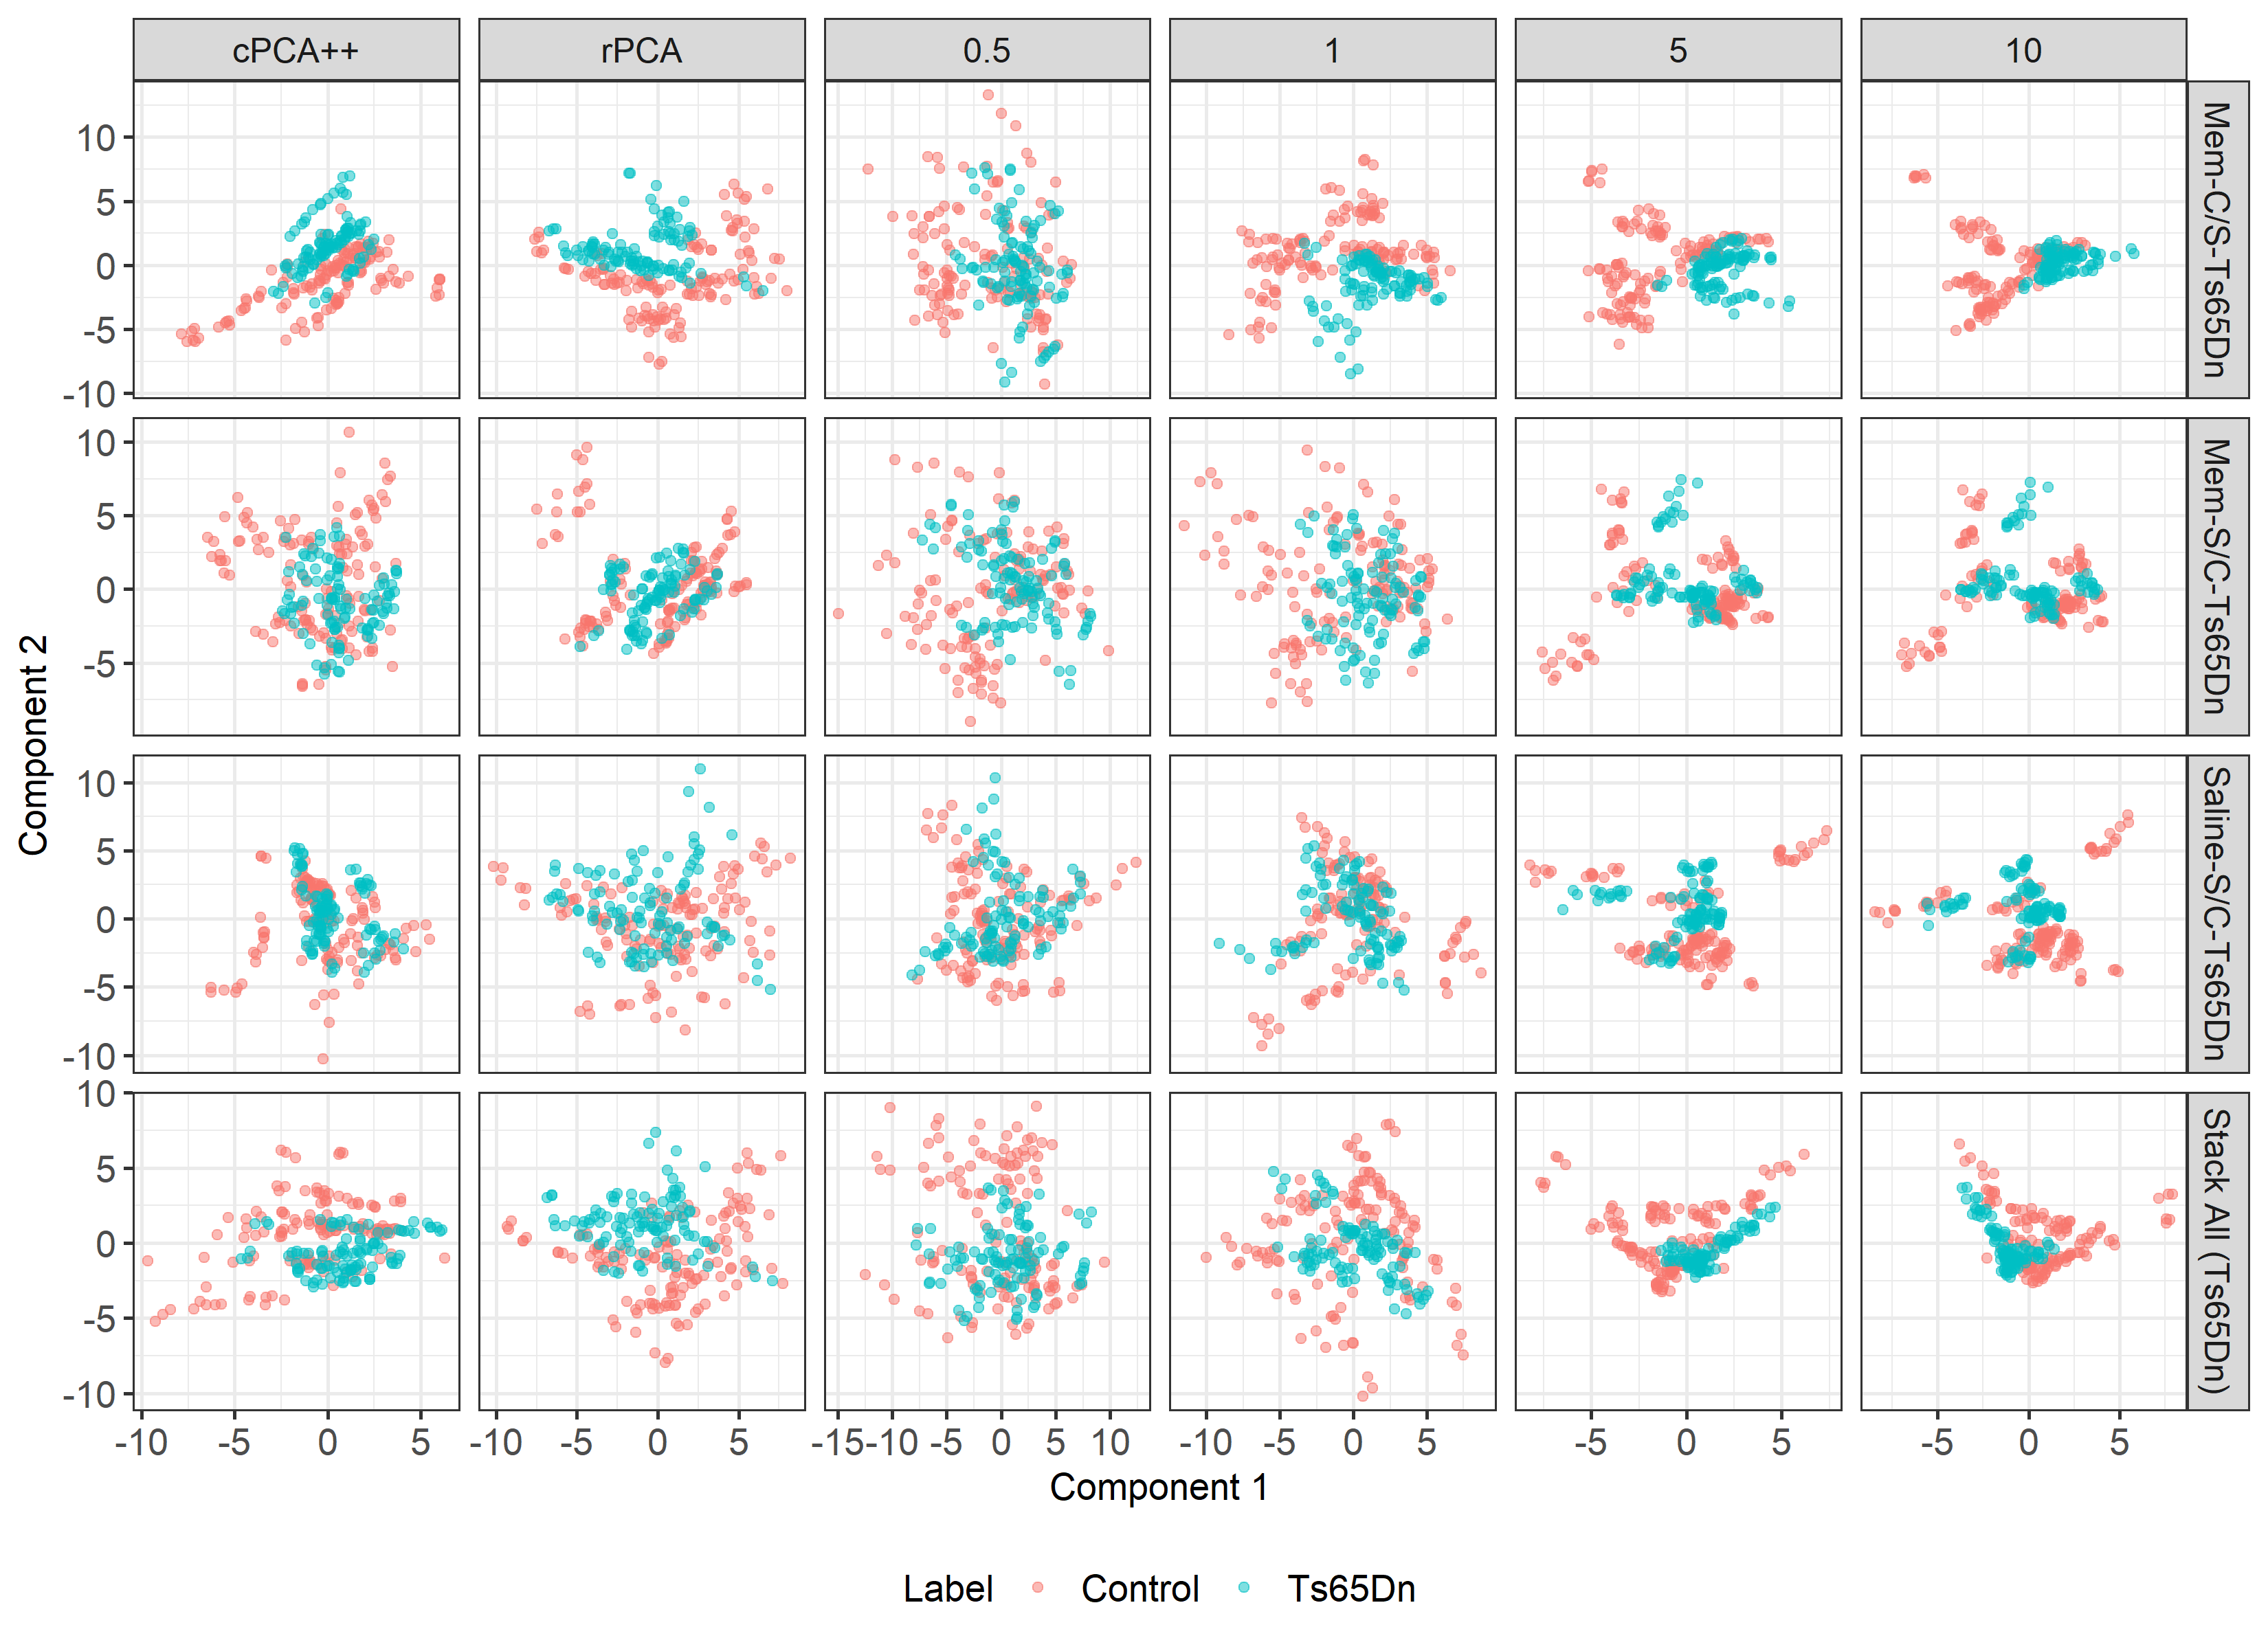
\includegraphics[width = 0.8\textwidth]{figure/Mouse_stack_cpc_rpcTs65Dn.png}
 %   \caption{Mouse Protein Expression Dataset}
 %   \label{fig:mouse_stack_cpca}
 % \end{figure}

% \begin{figure}[!ht]
%   \centering
%   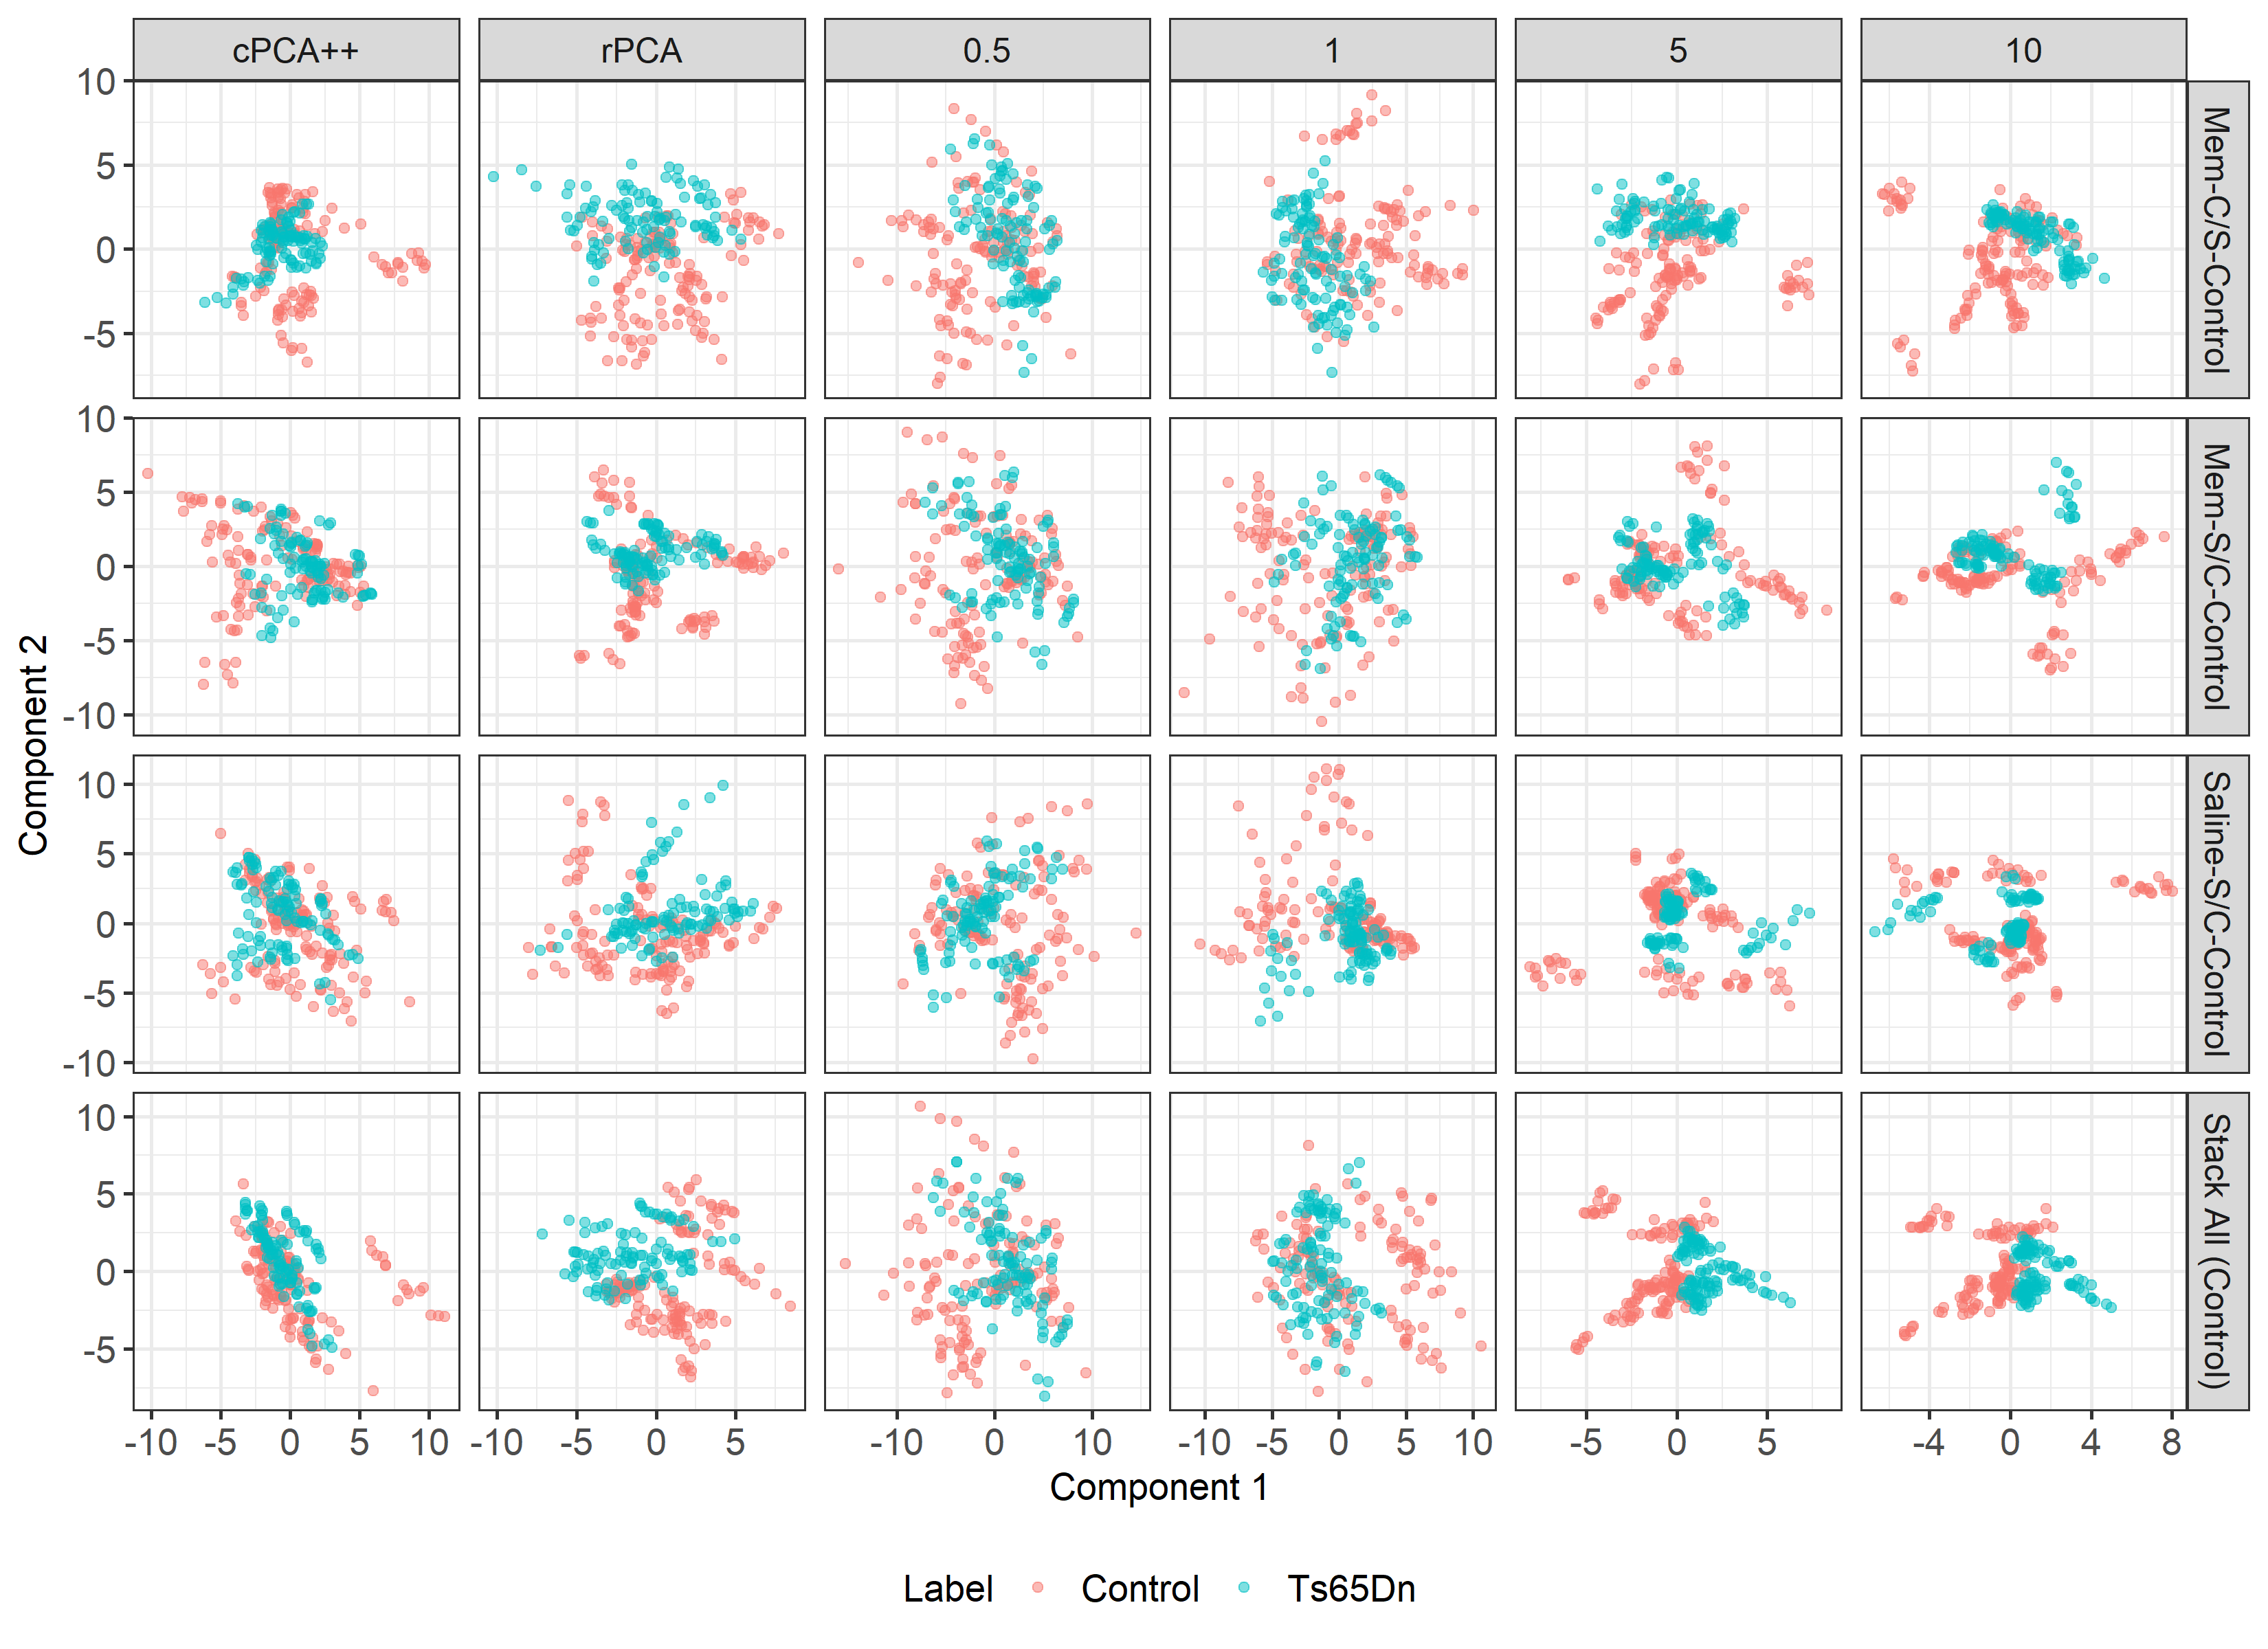
\includegraphics[width = 0.8\textwidth]{figure/Mouse_stack_cpc_rpcControl.png}
%   \caption{Mouse Protein Expression Dataset}
%   \label{fig:mouse_control_vary}
% \end{figure}

% \begin{figure}[!ht]
%   \centering
%   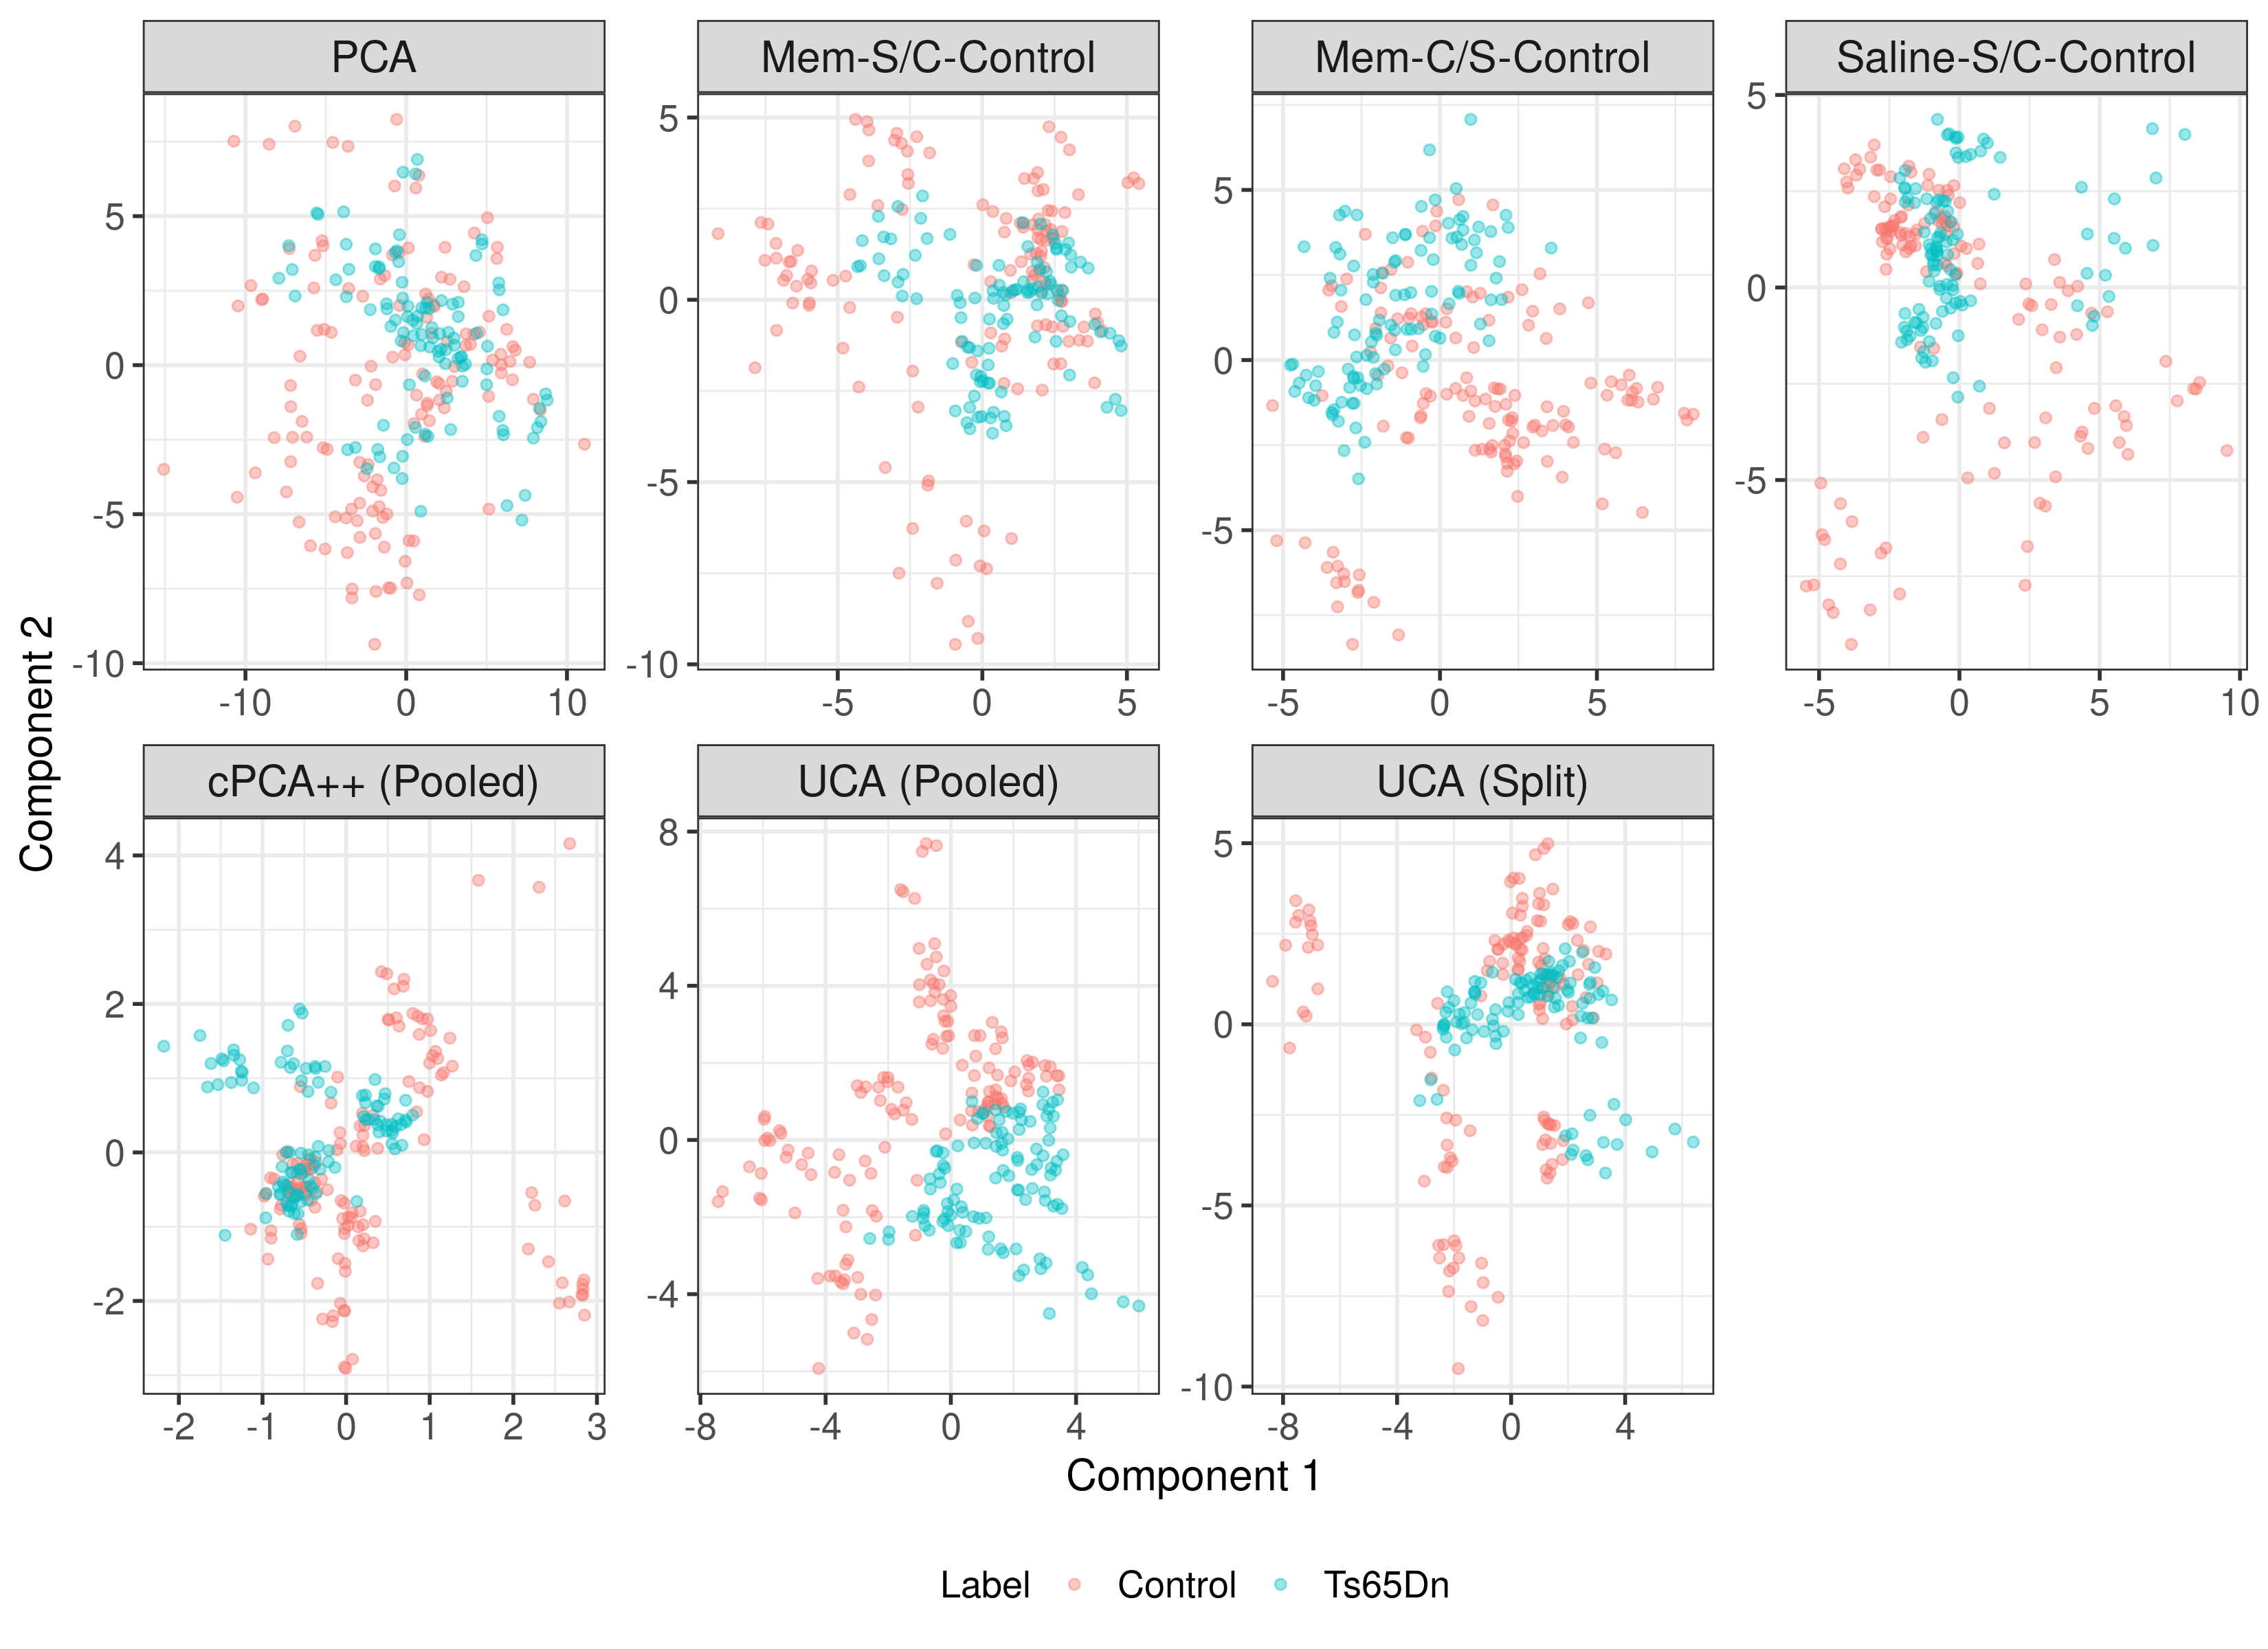
\includegraphics[width = 0.8\textwidth]{figure/Mouse_split_stack_Control.png}
%   \caption{Mouse Protein Expression Dataset}
%   \label{fig:mouse_stack_control}
% \end{figure}

\end{document}


%%% TO DO %%%
%\textbf{since some of the colors in the PCA are too similar, I had another idea, do you think we can do shapes as well? So like the ``bad'' emotions (anger, digust, etc.) get different shapes?}
% Discussion rewrite
% structure of methods argument

%%% Things to think about %%%
% an interpretation for $\lambda$
% are our solutions unique? why force v^T Bv  = 1, not 0.25 or 2. does the result give us the same eigenvectors but scaled eigenvalues? 
% if you scale the constraint does the estimated v just a scaled version?
% I.e. does it just live in the same space? Maybe the direction wouldn't change

